\documentclass[presentation]{beamer}
\usetheme{CambridgeUS}
\usecolortheme{orchid}

\definecolor{themeColor}{HTML}{1dc600}

\setbeamercolor*{structure}{bg=black,fg=themeColor}

\setbeamercolor*{palette primary}{use=structure,fg=white,bg=structure.fg}
\setbeamercolor*{palette secondary}{use=structure,fg=white,bg=structure.fg!75}
\setbeamercolor*{palette tertiary}{use=structure,fg=white,bg=structure.fg!50!black}
\setbeamercolor*{palette quaternary}{fg=white,bg=black}

\setbeamercolor{section in toc}{fg=black,bg=white}
\setbeamercolor{alerted text}{use=structure,fg=structure.fg!50!black!80!black}

\setbeamercolor{titlelike}{parent=palette primary,fg=structure.fg!50!black}
\setbeamercolor{frametitle}{bg=structure.fg!10!white,fg=structure.fg!50!black!80!black}

\setbeamercolor*{titlelike}{parent=palette primary}

\usepackage[utf8]{inputenc}
\usepackage{amssymb}
\usepackage{graphicx}
\usepackage{subfigure}
\usepackage{multirow}
\usepackage{hhline}
\usepackage{amsfonts,amstext,amssymb,wasysym}
\usepackage{fancyvrb}
\usepackage{alltt}
\usepackage{textcomp}
\usepackage{url}
\usepackage{multimedia,pgf}
\usepackage{geometry}
\usepackage{minted}
\usepackage{bibentry}
\usepackage{framed}
\usepackage{cleveref}
\nobibliography*

\title[Continuous integration and delivery]{Continuous integration and delivery \\ \scriptsize{A quick guide through the wonders of teamwork with distributed version control systems, dependency management, build automation, and continuous integration and delivery.}}

\author[Pianini]{
Danilo Pianini\\
\texttt{{\footnotesize danilo.pianini@unibo.it}}}


\institute[UniBo]
{\textsc{Alma Mater Studiorum}---Universit\`a di Bologna a Cesena}

\date[\today{}]{Paradigmi di Programmazione e Sviluppo \\
\scriptsize \today{} - Cesena (Italy)
}

\pgfdeclareimage[height=0.625cm]{university-logo}{images/logo}
\logo{\pgfuseimage{university-logo}}


\begin{document}

\AtBeginSubsection[]{%
  \begin{frame}<beamer>
    \frametitle{Outline}
    \tableofcontents[currentsection,currentsubsection]
  \end{frame}
  \addtocounter{framenumber}{-1}% If you don't want them to affect the slide number
}

%===============================================================================
\frame[label=coverpage]{\titlepage}
%===============================================================================

%===============================================================================
%===============================================================================
\section*{Outline}
%===============================================================================
%===============================================================================

\frame{\tableofcontents}

%===============================================================================
%===============================================================================
\section{Introduction}
\begin{frame}[fragile, allowframebreaks]{Why continuous?}
	\begin{block}{Avoid the integration hell}
		\begin{itemize}
			\item Work in parallel
			\item Don't waste developers' time with repetitive tasks
			\item Don't break stuff
		\end{itemize}
		Time is money
	\end{block}
	\begin{itemize}
		\item Software development used to take several months for ``integrating'' a couple of years of development \cite{fowlerci}
		\item Historically introduced by the extreme programming (XP) community
		\item Today used by companies that do not adopt XP
		\item IMVU \cite{imvu} delivers its software up to 50 times \textbf{per day}
		\item Google and Mozilla release \textbf{at least} once a day
	\end{itemize}
	\begin{block}{Higher frequency, lower risk \cite{semaphoreci}}
		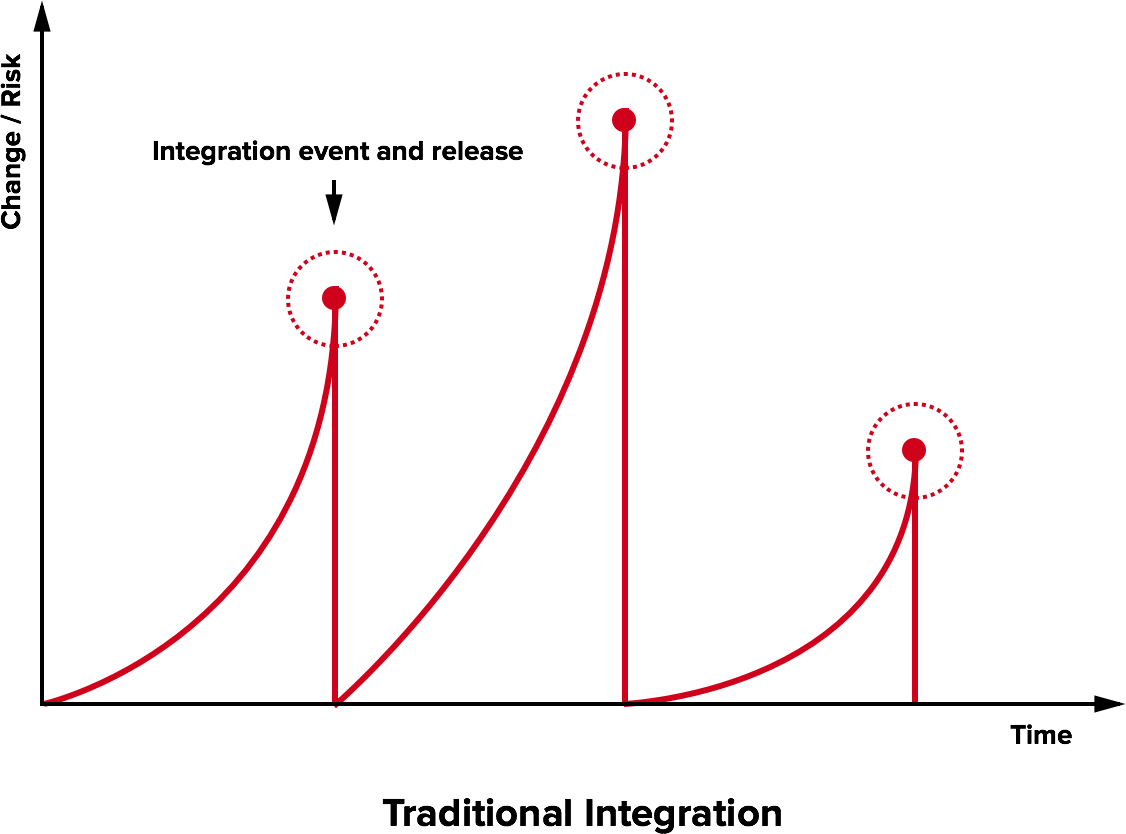
\includegraphics[width=.49\textwidth]{images/integration-traditional}
		~ \vline ~
		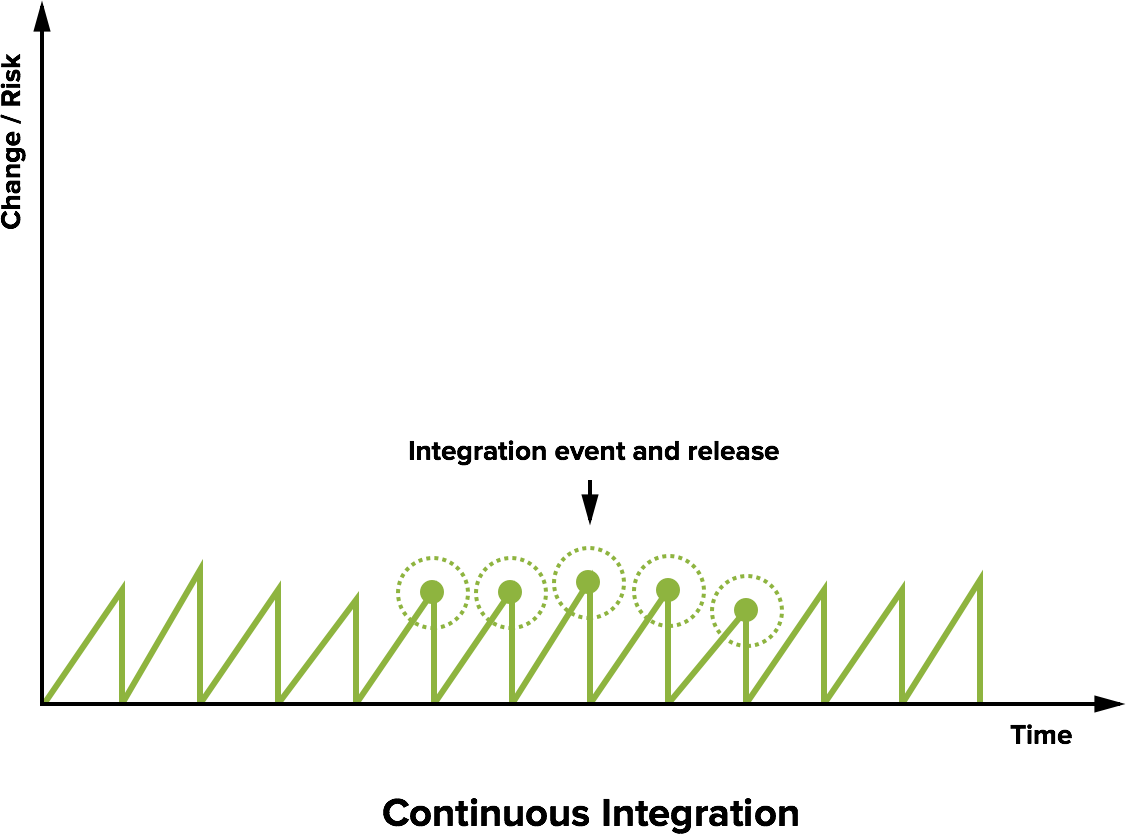
\includegraphics[width=.49\textwidth]{images/integration-continuous}
	\end{block}
\end{frame}

\subsection{Highway to hell}

\newcommand{\baddev}[0]{Jimmy}
\newcommand{\gooddev}[0]{Elliot}

\begin{frame}[fragile, allowframebreaks]{What could possibly go wrong? Welcome to Hell }
	\baddev{} \cite{jargon} and \gooddev{} develop a software project together.
	\begin{block}{Diverging histories}
		\begin{itemize}
			\item \baddev{} must develop a new feature, picks the latest \gooddev{}'s code
			\item \baddev{} begins, and in the meantime \gooddev{} goes on with the rest
			\item \baddev{} completes his part
			\item \baddev{}'s code does not work the latest version
		\end{itemize}
		\textbf{Keep your code in sync with the main development line}
	\end{block}
	\begin{block}{It was working two minutes ago}
		\begin{itemize}
			\item \baddev{} developed a new feature and tests it
			\item \baddev{} shows the feature five minutes later to \gooddev{}, it does not work anymore
			\item \baddev{} can't figure out what happened, and needs to spend time debugging
			\item \gooddev{} can't see the feature, and must wait for \baddev{} to iron the problem out
		\end{itemize}
		\textbf{Make sure you can restore any small change you made}
	\end{block}
	\begin{block}{Stylish hell}
		\begin{itemize}
			\item \baddev{} and \gooddev{} styles are misaligned
			\begin{itemize}
				\item CRLF vs. LF
				\item Egyptian parentheses \cite{jargon} vs. Allman
				\item Tabs vs. spaces
				\item Basically anything you can start a religion war upon
			\end{itemize}
			\item \baddev{} and \gooddev{} IDEs are configured differently
			\item The project continuously flips from one style to the other, inconsistently
			\item Becomes impossible to localize changes
		\end{itemize}
		\textbf{Agree on style (possibly using existing shared conventions), and enforce its adoption}
	\end{block}
	\begin{block}{Tests as decorations}
		\begin{itemize}
			\item \baddev{} prepared a lot of nice tests
			\item \baddev{} rarely executes them
			\item \baddev{} code ends up being broken
		\end{itemize}
		\textbf{Execute your tests for every change you make}
	\end{block}
	\begin{block}{Works on my PC}
		\begin{itemize}
			\item Tests run correctly on \baddev{} computer
			\item They don't on \gooddev{}'s
			\item Time gets wasted to debug the tests to decide whether or not the code should get debugged
		\end{itemize}
		\textbf{Execute your tests in a fresh environment resembling the production environment}
	\end{block}
	\begin{block}{Unexpected merge failure}
		\begin{itemize}
			\item \baddev{} develops a new feature, everything seems to work
			\item The feature gets merged with the mainline
			\item Tests fail
		\end{itemize}
		\textbf{Test the integration before performing it}
	\end{block}
	\begin{block}{Dependency hell}
		\begin{itemize}
			\item \baddev{} needs a library
			\item Imports it directly in the code base
			\item This dependency now must be dealt with manually:
			\begin{itemize}
				\item Updates
				\item Bugfixes
				\item Dependency's dependencies
			\end{itemize}
			\item Big projects can very easily require hundreds of libraries
		\end{itemize}
		\textbf{Automatize the dependency management}
	\end{block}
	\begin{block}{Fermented build}
		\begin{itemize}
			\item The project builds correctly and passes al tests
			\item Nobody touches it, nobody builds it again for weeks
			\item Once a rebuild is required, the project no longer builds or passes tests
		\end{itemize}
		\textbf{Rebuild often}
	\end{block}
\end{frame}

\begin{frame}[fragile, allowframebreaks]{What could possibly get improved? Road to paradise}
	\begin{block}{Protoduction \cite{jargon}}
		\begin{center}
			
\includegraphics[width=.25\textwidth]{images/protoduction} \\
			When prototype code ends up in production
		\end{center}
		\begin{itemize}
			\item Classically used with a negative meaning
			\item It's time to rehabilitate it
		\end{itemize}
		\textbf{Make it easy to access and use the latest prototype}
	\end{block}
	\begin{block}{It's compiling \cite{xkcd303}}
		\centering
		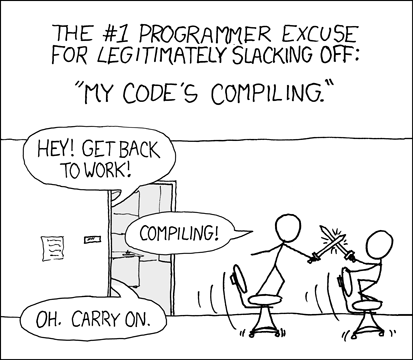
\includegraphics[width=.49\textwidth]{images/compiling}

		\textbf{Make the building process fast!}
	\end{block}
	\begin{block}{It's delivering}
		\begin{itemize}
			\item Business Analysis often need the latest version of the software do demonstrate upcoming features
			\item \baddev{}'s time gets is spent several times per week just for preparing alpha releases
		\end{itemize}
		\textbf{Automatize the delivery}
	\end{block}
\end{frame}

\subsection{Stairway to heaven}

\begin{frame}[fragile]{Summary}
	\begin{itemize}
		\item Keep feature code in sync with the mainline
		\item Make sure you can restore any small change you make
		\item Agree and enforce a style (and report problems)
		\item Execute all tests for every change
		\item Execute your tests on a freshly prepared machine resembling production
		\item Test the integration before integrating
		\item Automatize the dependency management
		\item Rebuild often
		\item Automatize the delivery
		\item Make the development artifacts available
		\item All the above, make it fast (non functional!)
	\end{itemize}
\end{frame}

\begin{frame}[fragile]{No silver bullet}
	\begin{itemize}
		\item No single magic solution to all these problems is available
		\item But they can all be tackled with the right combination of:
		\begin{itemize}
			\item Development tools
			\item Development methodologies
			\item Automatization tools
		\end{itemize}
	\end{itemize}
\end{frame}

\begin{frame}[fragile, allowframebreaks]{Our bullets}
	\begin{block}{git}
		\begin{center}
			
\includegraphics[height=.1\textheight]{images/git}
		\end{center}
		
		A distributed version control system. Will help with:
		\begin{itemize}
			\item Keep feature code in sync with the mainline
			\item Make sure you can restore any small change you make
			\item All the above, make it fast!
		\end{itemize}
	\end{block}
	\begin{block}{git-flow}
		A methodology for team development using git. Will help with:
		\begin{itemize}
			\item Keep feature code in sync with the mainline
			\item Test the integration before integrating
		\end{itemize}
	\end{block}
	\begin{block}{GitHub}
		\begin{center}
			
\includegraphics[height=.1\textheight]{images/github-logo}
		\end{center}
		
		A git repository hosting with support for forking, pull requesting and code reviewing. Will help with:
		\begin{itemize}
			\item Keep feature code in sync with the mainline
			\item Test the integration before integrating
			\item Make the development artifacts available
		\end{itemize}
	\end{block}
	\begin{block}{PMD, CPD, FindBugs, Checkstyle, Scalastyle, Scalameta, Scapegoat...}
		\begin{center}
			
\includegraphics[height=.1\textheight]{images/pmd-logo} ~
			
\includegraphics[height=.1\textheight]{images/checkstyle-logo} ~
			
\includegraphics[height=.1\textheight]{images/findbugs} ~
		\end{center}
		
		Code quality checkers. Will help with:
		\begin{itemize}
			\item Agree and enforce a style (and report problems)
		\end{itemize}
	\end{block}
	\begin{block}{Gradle}
		\begin{center}
			
\includegraphics[height=.1\textheight]{images/gradle-logo}
		\end{center}
		
		Dependency manager and build automation tool. Will help with:
		\begin{itemize}
			\item Agree and enforce a style (and report problems)
			\item Execute all tests for every change
			\item Automatize the delivery
			\item All the above, make it fast!
		\end{itemize}
	\end{block}
	\begin{block}{Travis CI (+ Docker)}
		\begin{center}
			
\includegraphics[height=.1\textheight]{images/travis-logo} ~ 
			
\includegraphics[height=.1\textheight]{images/docker-logo} ~ 
		\end{center}

		Continuous integration and delivery system (+ software container). Will help with:
		\begin{itemize}
			\item Execute all tests for every change
			\item Execute your tests on a freshly prepared machine resembling production
			\item Test the integration before integrating
			\item Rebuild often
			\item Automatize the delivery
			\item All the above, make it fast!
		\end{itemize}
	\end{block}
	\begin{block}{Maven Central, Bintray, Surge.sh, Heroku, Azure, S3...}
		\begin{center}
			
\includegraphics[height=.08\textheight]{images/central-logo} \\ 
			
\includegraphics[height=.1\textheight]{images/bintray-logo} ~ 
 			
\includegraphics[height=.1\textheight]{images/surge-logo} ~ 
%  			
\includegraphics[height=.1\textheight]{images/heroku-logo} ~ 
%  			
\includegraphics[height=.1\textheight]{images/azure-logo} ~ 
 			
\includegraphics[height=.1\textheight]{images/s3-logo} ~ 
		\end{center}

		Software Distributors. Will help with:
		\begin{itemize}
			\item Make the development artifacts available
		\end{itemize}
	\end{block}
\end{frame}

\begin{frame}[fragile]{Spoiler: the complete process}
	\begin{center}
		\includegraphics[width=.9\textwidth]{images/ci}
	\end{center}
\end{frame}

%===============================================================================
%===============================================================================
\section{Successful teamwork with distributed control version systems}
%===============================================================================
%===============================================================================

%===============================================================================
\subsection{git}
%===============================================================================

\begin{frame}[fragile]{How will the world look like shortly}
	\begin{center}
		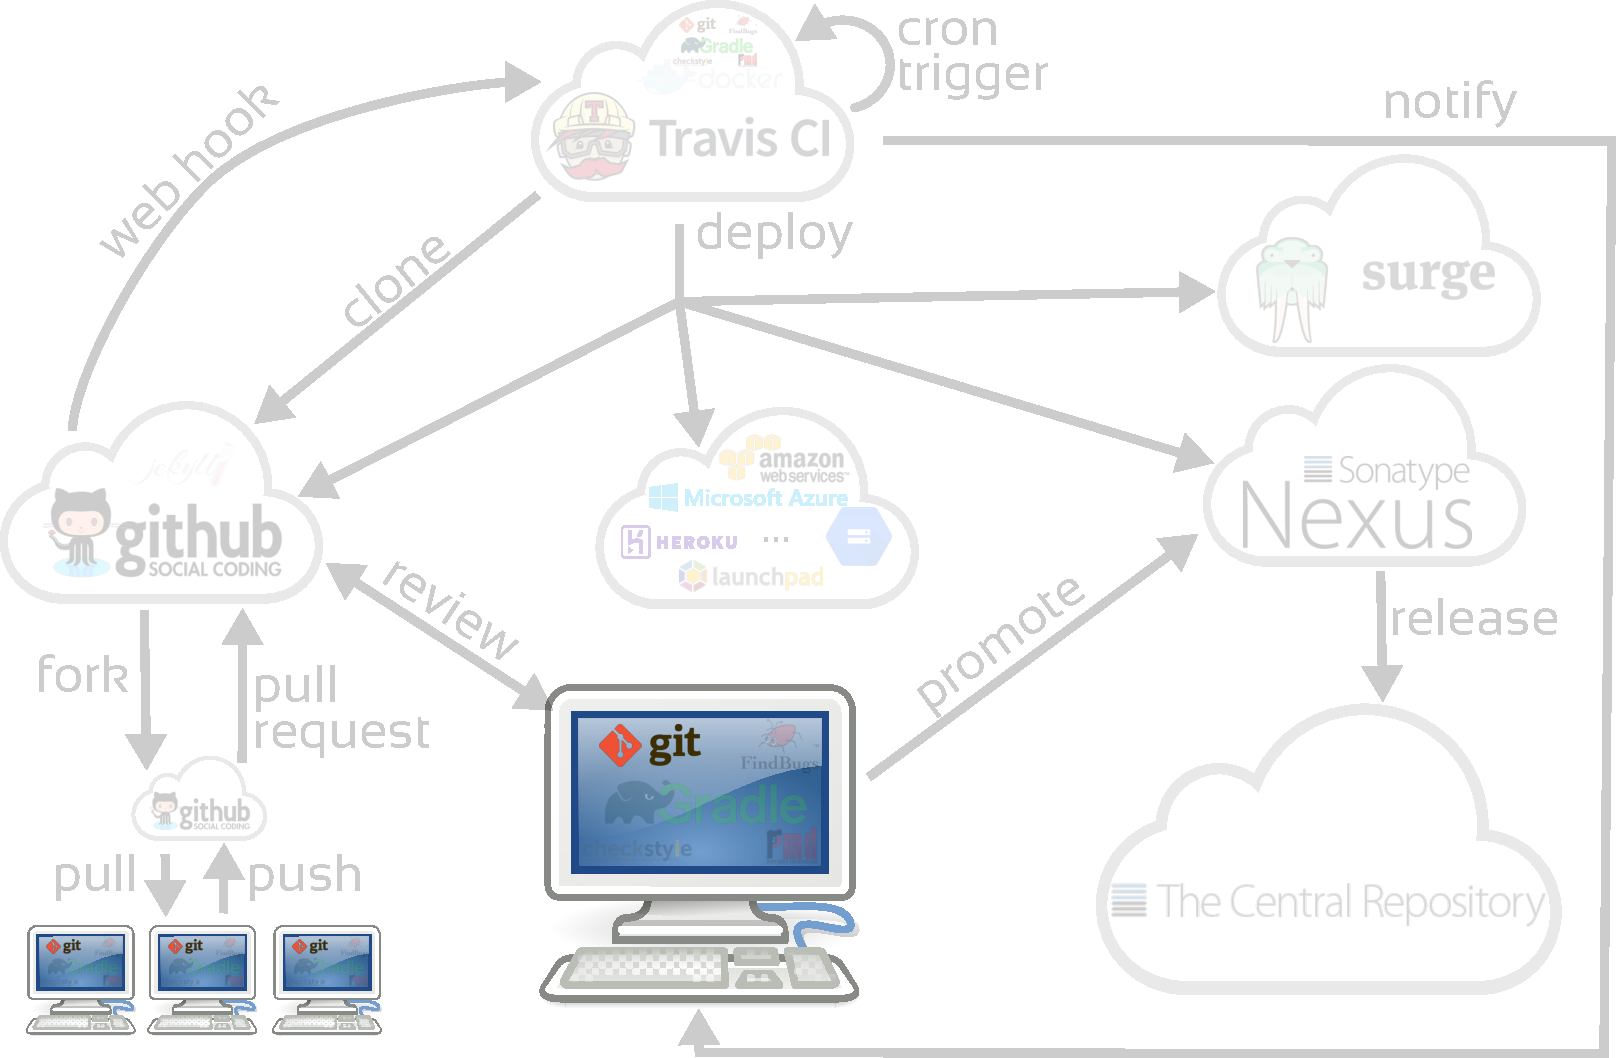
\includegraphics[width=.9\textwidth]{images/ci-git}
	\end{center}
\end{frame}

\begin{frame}[fragile]{Bits of history}
	\begin{itemize}
		\item In April 2005, BitKeeper, the SCM Linux was developed with, withdrawn the free (as in beer) use
		\item No other SCM met the requirements of Torvalds
		\begin{itemize}
			\item Performance was the \textit{real} issue with such a code base
		\end{itemize}
		\item Torvalds decided to write his own
		\item The project was successful, and Torvalds appointed maintenance to Hamano
	\end{itemize}
	\begin{block}{Why the name}
		\begin{quote}
			I'm an egotistical bastard, and I name all my projects after myself. First 'Linux', now 'git'. \footnote{\tiny{From the project Wiki. ``git'' is slang for ``pig headed, think they are always correct, argumentative''}}
			\begin{flushright}
				\normalfont{--- Linus Torvalds}
			\end{flushright}
		\end{quote}
	\end{block}
\end{frame}

\begin{frame}[fragile]{The \texttt{git} \texttt{README.md} file}
	\begin{block}{}
		\begin{minted}[fontsize=\footnotesize]{yaml}
GIT - the stupid content tracker

"git" can mean anything, depending on your mood.

 - random three-letter combination that is pronounceable, and not
   actually used by any common UNIX command.  The fact that it is a
   mispronounciation of "get" may or may not be relevant.
 - stupid. contemptible and despicable. simple. Take your pick from the
   dictionary of slang.
 - "global information tracker": you're in a good mood, and it actually
   works for you. Angels sing, and a light suddenly fills the room. 
 - "goddamn idiotic truckload of sh*t": when it breaks
		\end{minted}
	\end{block}
\end{frame}

\begin{frame}[fragile]{Features}
	\begin{itemize}
		\item UNIX-oriented: tracks stuff like UNIX file permits.
		\item Distributed development (the whole development history is copied locally)
		\item Diff-based history tracking
		\item Implicit file naming (history preserved on renames)
		\item Very strong support to non-linear development
		\item Written in C
		\item Approximately 10 times faster than Mercurial, 100 times faster than other DVCS (e.g. Bazaar)
		\item Uses existing protocols (ssh, http, ftp, rsync...)
		\item Pluggable merge strategies (defaults to recursive three-ways merge or octopus for 3+ heads)
	\end{itemize}
\end{frame}

\begin{frame}[fragile, allowframebreaks]{The compact guide to git}
	Sub-commands in \texttt{typewritertext}, concepts in \textit{italic}.
	\begin{block}{\texttt{init}}
		Initializes a new repository
	\end{block}
	\begin{block}{\textit{Stage}}
		\begin{center}
			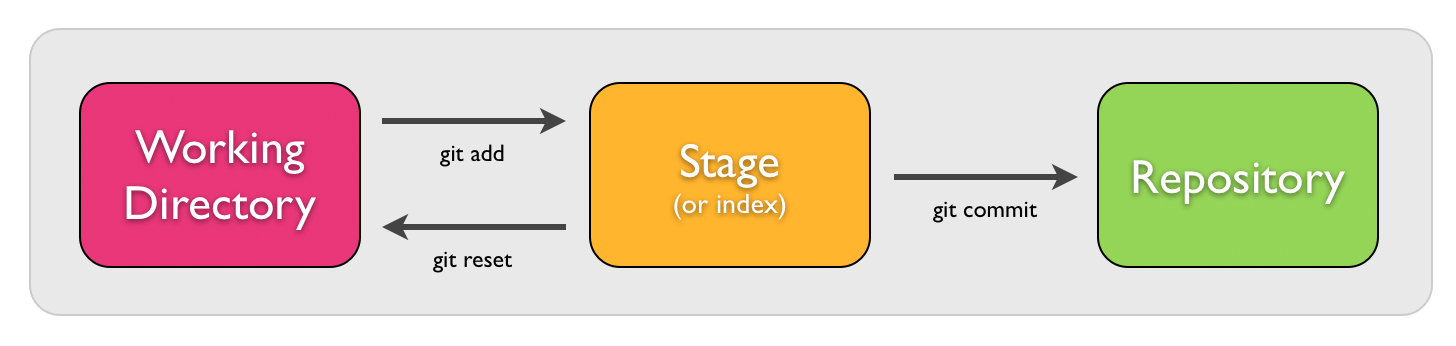
\includegraphics[width=.5\textwidth]{images/staging}
		\end{center}
		The place where git stores the files whose changes will be saved next
	\end{block}
	\begin{block}{\texttt{add} / \texttt{reset}}
		Moves/Removes files onto/from the \textit{stage}
	\end{block}
	\begin{block}{.gitignore}
		A file listing the pathspecs that git should ignore even if added
	\end{block}
	\begin{block}{\texttt{commit}}
		Create a new ``snapshot'' (it's actually a changeset) with the contents of the \textit{stage}
	\end{block}
	\begin{block}{\texttt{tag}}
		Associates a symbolic name and message to a commit.
	\end{block}
	\begin{block}{\textit{HEAD}}
		The pointer to the current changeset (commits)
	\end{block}
	\begin{block}{\textit{Branch}}
		\begin{center}
			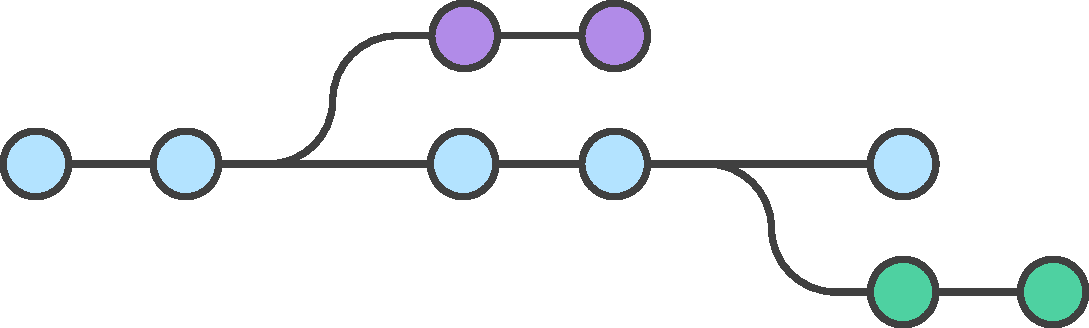
\includegraphics[width=.5\textwidth]{images/branches}
		\end{center}
		A named development line.
	\end{block}
	\begin{block}{\textit{master}}
		The name of the default development line.
	\end{block}
	\begin{block}{\texttt{checkout}}
		Moves the \texttt{HEAD} across commits.
		Can be used to switch branches or create new ones (\texttt{checkout -b}).
		If the commit is not the latest (in the current \textit{branch}), git switches to \textit{detached head} mode.
	\end{block}
	\begin{block}{\texttt{branch}}
		Lists the existing branches. Can delete them (\texttt{branch -d}).
	\end{block}
	\begin{block}{\texttt{merge}}
		Unifies a target branch with the current branch, merging the changes and creating a new commit.
		The merging algorithm is configurable.
		In case of conflicts, they must be manually solved.
	\end{block}
	\begin{block}{\textit{fast forward}}
		The operation executed by default when a merge is requested and a branch is simply behind another.
	\end{block}
	\begin{block}{\texttt{remote}}
		Configures the (possibly remote) locations where copies of this repository exist.
	\end{block}
	\begin{block}{\textit{upstream}}
		The \textit{remote} where to execute the remote operation against if not otherwise specified.
	\end{block}
	\begin{block}{\texttt{clone}}
		Copies a repository from a possibly remote location.
		Alternative to \texttt{init}.
		Automatically sets the \textit{upstream} to the cloned location.
	\end{block}
	\begin{block}{\texttt{fetch}}
		Locally copies the changes from an URL or a configured \textit{remote}.
	\end{block}
	\begin{block}{\texttt{pull}}
		Equivalent to \texttt{fetch}+\texttt{merge}.
	\end{block}
	\begin{block}{\texttt{push}}
		Copies the local changes to an URL or a configured remote.
		A configured remote can be set as upstream (\texttt{push -u}).
	\end{block}
\end{frame}

\begin{frame}[fragile, allowframebreaks]{Best practices with git}
	\begin{block}{Prefer the terminal}
		Do not use graphical interfaces to the DVCS until you have a complete grasp of it, only rely on the terminal.
	\end{block}
	\begin{block}{Ignore list}
		Immediately configure a \texttt{.gitignore} file
	\end{block}
	\begin{block}{Choose what to track carefully}
		Track only the files that are not generable (sources, resources, scripts...). Never ever track
		\begin{itemize}
			\item binaries
			\item generated sources (e.g. from ANTLR, Xtend, JavaCC...)
			\item generable documentation (e.g. Javadocs)
			\item libraries (if you have a dependency manager)
		\end{itemize}
		Failing at doing so will make your repository \textbf{explode} in size.
	\end{block}
	\begin{block}{Properly configure the behaviour with newlines}
		\begin{itemize}
			\item The default behaviour is inconsistent between Windows and UNIX, and you may end up with a mixture
			\item Force the end line of your choice (may your choice be LF)
			\item Disable the autoclrf conversion, frequently use \texttt{diff} to make sure you're not messing up
		\end{itemize}
	\end{block}
\end{frame}

\begin{frame}[fragile]{How the world looks like now}
	\begin{center}
		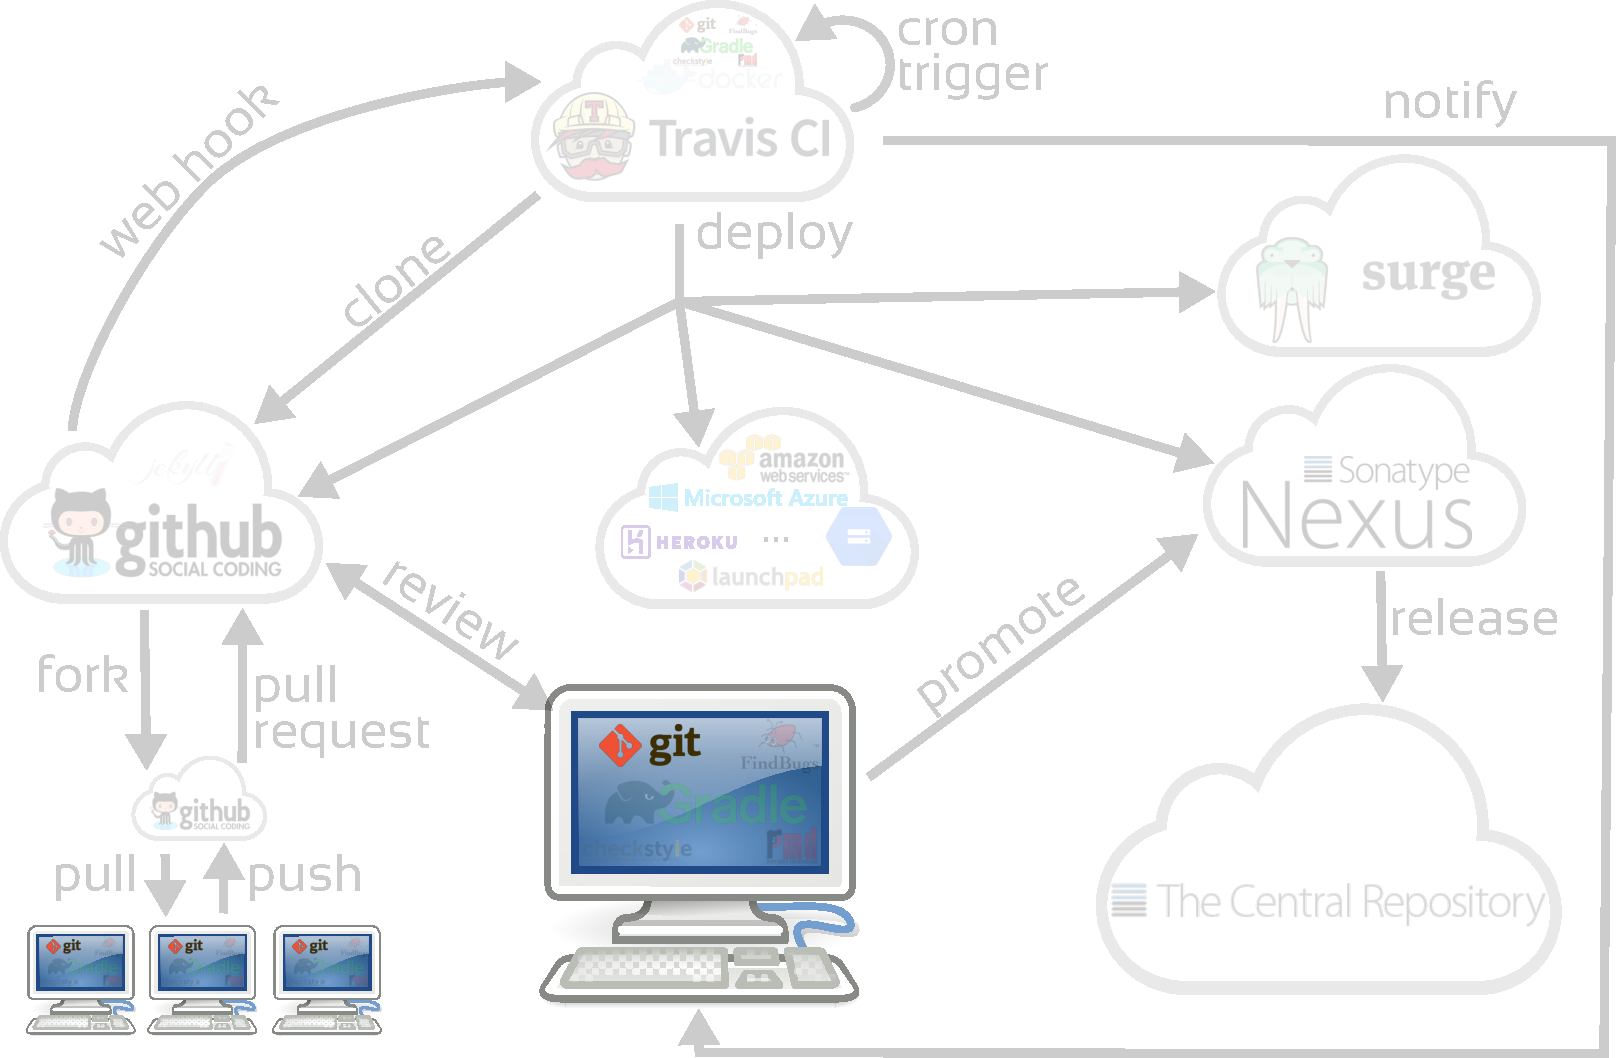
\includegraphics[width=.9\textwidth]{images/ci-git}
	\end{center}
\end{frame}


%===============================================================================
\subsection{git flow}
%===============================================================================

\begin{frame}[fragile]{How will the world look like shortly}
	\begin{center}
		\includegraphics[width=.9\textwidth]{images/ci-gitflow}
	\end{center}
\end{frame}

\begin{frame}[fragile]{Git Flow as a development model}
	\begin{columns}
		\begin{column}{.53\textwidth}
			\begin{itemize}
				\item Mainline branch: \texttt{master}
				\begin{itemize}
					\item Always alive
				\end{itemize}
				\item Development branch: \texttt{develop}
				\begin{itemize}
					\item Branches from \texttt{master}
					\item Never merges
				\end{itemize}
				\item New feature: \texttt{feature-*}
				\begin{itemize}
					\item Branches from and merges to \texttt{develop}
				\end{itemize}
				\item New release: \texttt{release-*}
				\begin{itemize}
					\item Branches from \texttt{develop}
					\item Merges to \texttt{master} and \texttt{develop}
					\item Creates a new version
				\end{itemize}
				\item Fix a bug on mainline: \texttt{hotfix-*}
				\begin{itemize}
					\item Branches from \texttt{master}
					\item Merges to \texttt{master} and \texttt{develop}
					\item Creates a new version
				\end{itemize}
			\end{itemize}
		\end{column}
		\begin{column}{.47\textwidth}
			\begin{center}
				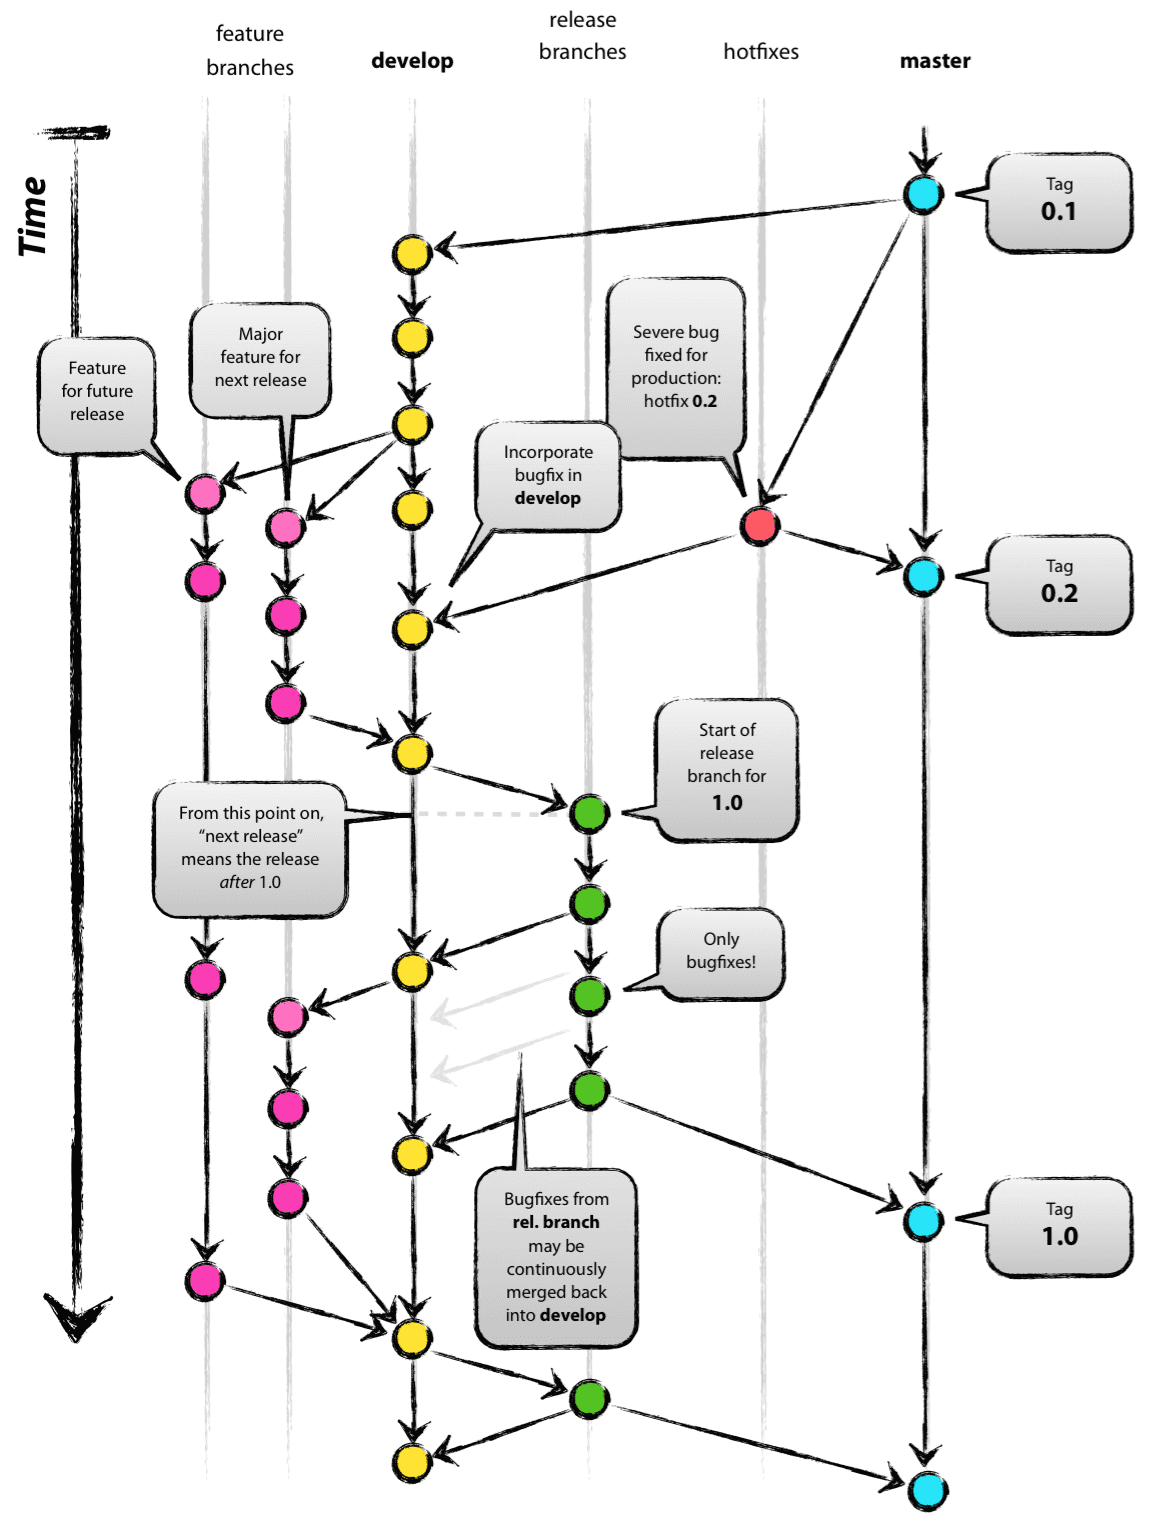
\includegraphics[width=\textwidth]{images/gitflow}
			\end{center}
		\end{column}
	\end{columns}
\end{frame}

\begin{frame}[fragile]{Developing new features}
	When a new feature must be added to the software, the team responsible for it should branch a \texttt{feature-myfeature} branch from \texttt{develop}.
	\begin{itemize}
		\item \texttt{git checkout -b feature-myfeature develop}
	\end{itemize}
	Once all the work has been done, the branch should get merged in \texttt{develop} and deleted. Even if fast-forward, the merge should be visible, to prevent history loss.
	\begin{itemize}
		\item \texttt{git checkout develop}
		\item \texttt{git merge --no-ff feature-myfeature}
		\item \texttt{git branch -d feature-myfeature}
	\end{itemize}
	In order to minimize the merging effort, it is a good practice to incorporate changes from \texttt{develop} from time to time (e.g. when another team completed another feature).
\end{frame}

\begin{frame}[fragile]{Releasing a new version}
	When the status of the \texttt{develop} branch is (besides the very last bits) the status of the next production release, a \texttt{release-version} should branch from \texttt{develop}.
	\begin{itemize}
		\item \texttt{git checkout -b release-version develop}
	\end{itemize}
	In this branch, only things like version number changes or last minute bug fixes should get incorporated. Once done, we merge the \texttt{release-version} branch back into \texttt{develop}...
	\begin{itemize}
		\item \texttt{git checkout develop}
		\item \texttt{git merge --no-ff release-version}
	\end{itemize}
	...and \texttt{master}. Plus, we tag master, so that we keep a reference to the exact repository status at release time. Then, we delete the \texttt{release-version} branch.
	\begin{itemize}
		\item \texttt{git checkout master}
		\item \texttt{git merge --no-ff release-version}
		\item \texttt{git tag -a version}
		\item \texttt{git branch -d release-version}
	\end{itemize}
\end{frame}

\begin{frame}[fragile]{Fix severe bugs affecting the mainline}
	You spot a bug in your current production branch. The fix must be delivered immediately.
	
	Start a new \texttt{hotfix-version} branch:
	\begin{itemize}
		\item \texttt{git checkout -b hotfix-version master}
	\end{itemize}
	Change the version number, fix the bug (also add a regression test). Once done, repeat the procedure already seen for a normal release.
	\begin{itemize}
		\item \texttt{git checkout develop}
		\item \texttt{git merge --no-ff hotfix-version}
		\item \texttt{git checkout master}
		\item \texttt{git merge --no-ff hotfix-version}
		\item \texttt{git tag -a version}
		\item \texttt{git branch -d hotfix-version}
	\end{itemize}
\end{frame}

\begin{frame}[fragile]{\texttt{git flow}}
	\begin{itemize}
		\item This workflow, first suggested by Vincent Driessen, got very popular.
		\item The command sequence is repetitive, and got automated
		\item A git extension (not part of the git distribution) is available:
		\begin{itemize}
			\item Introduces the \texttt{git flow} subcommand
			\item Starts and finishes feature, release, hotfix (and support)  branches
			\item Under the hood, it calls exactly the commands listed previously
		\end{itemize}
		\item My suggestion 
		\begin{itemize}
			\item \textit{learn} git flow as a development model
			\item Get acquainted with it using standard \texttt{git}
			\item When you are very confident that you know what the tool is doing with your repository, use \texttt{git flow}
			\item This is a good approach in general to new tools:
			\begin{itemize}
				\item understand the idea
				\item learn the basics
				\item understand what goes on under the hood
				\item use the advanced features productively
			\end{itemize}
		\end{itemize}
	\end{itemize}
\end{frame}

\begin{frame}[fragile]{How the world looks like now}
	\begin{center}
		\includegraphics[width=.9\textwidth]{images/ci-gitflow}
	\end{center}
\end{frame}

%===============================================================================
\subsection{GitHub}
%===============================================================================

\begin{frame}[fragile]{How will the world look like shortly}
	\begin{center}
		\includegraphics[width=.9\textwidth]{images/ci-fork}
	\end{center}
\end{frame}

\begin{frame}[fragile, allowframebreaks]{GitHub}
	\begin{block}{Main features}
		\begin{itemize}
			\item Support for Git repositories hosting
			\item Free for public, open source projects
			\item Issue tracker
			\item Support for defining teams / organizations
			\item Code highlighting
			\item History navigation
			\item Markdown formatting supported
			\item Fork/Pull request support
		\end{itemize}
	\end{block}
	\begin{block}{Static websites}
		\begin{center}
			
\includegraphics[height=.2\textheight]{images/jekyll-logo}
		\end{center}
		\begin{itemize}
			\item One static website per project, one per user, one per organization
			\begin{itemize}
				\item The \texttt{gh-pages} branch of each repository is implicitly considered a documentation web page
				\item Support for Jekyll! \footnote{\url{https://jekyllrb.com/}}
			\end{itemize}
		\end{itemize}
	\end{block}
	\begin{block}{Why GitHub}
		\begin{itemize}
			\item By far the largest host of source code in the world
			\item Markdown supported also in comments and issue posts
			\item Beautiful development statistics
			\item De facto standard for open source software
		\end{itemize}
	\end{block}
\end{frame}

%===============================================================================
\subsection{Working with forks}
%===============================================================================

\begin{frame}[fragile]{Back to centralized?}
	\begin{itemize}
		\item There is no inherent concept of ``central repository'' in git
		\item The Git flow branching model considers a ``central'' repository (truth repo) where every developer insists
		\item The methodology focusses on how to maintain the central repo, however:
		\begin{itemize}
			\item Each developer may have his own copy (fork) of the project
			\item There may be a responsible of the central repository, the only one with write permits
			\item Other developers request the maintainer to pull from their forks
			\begin{itemize}
				\item there is specific support for this workflow in hosting platforms
			\end{itemize}
			\item The maintainer decides when to actually create releases
		\end{itemize}
		\item In git, use \texttt{remote} to easily work with multiple forks
	\end{itemize}
\end{frame}

\begin{frame}[fragile]{How the world looks like now}
	\begin{center}
		\includegraphics[width=.9\textwidth]{images/ci-fork}
	\end{center}
\end{frame}

%===============================================================================
%===============================================================================
\section{Build automation}
%===============================================================================
%===============================================================================

%===============================================================================
\subsection{Dependency management}
%===============================================================================

\begin{frame}[fragile]{How will the world look like shortly}
	\begin{center}
		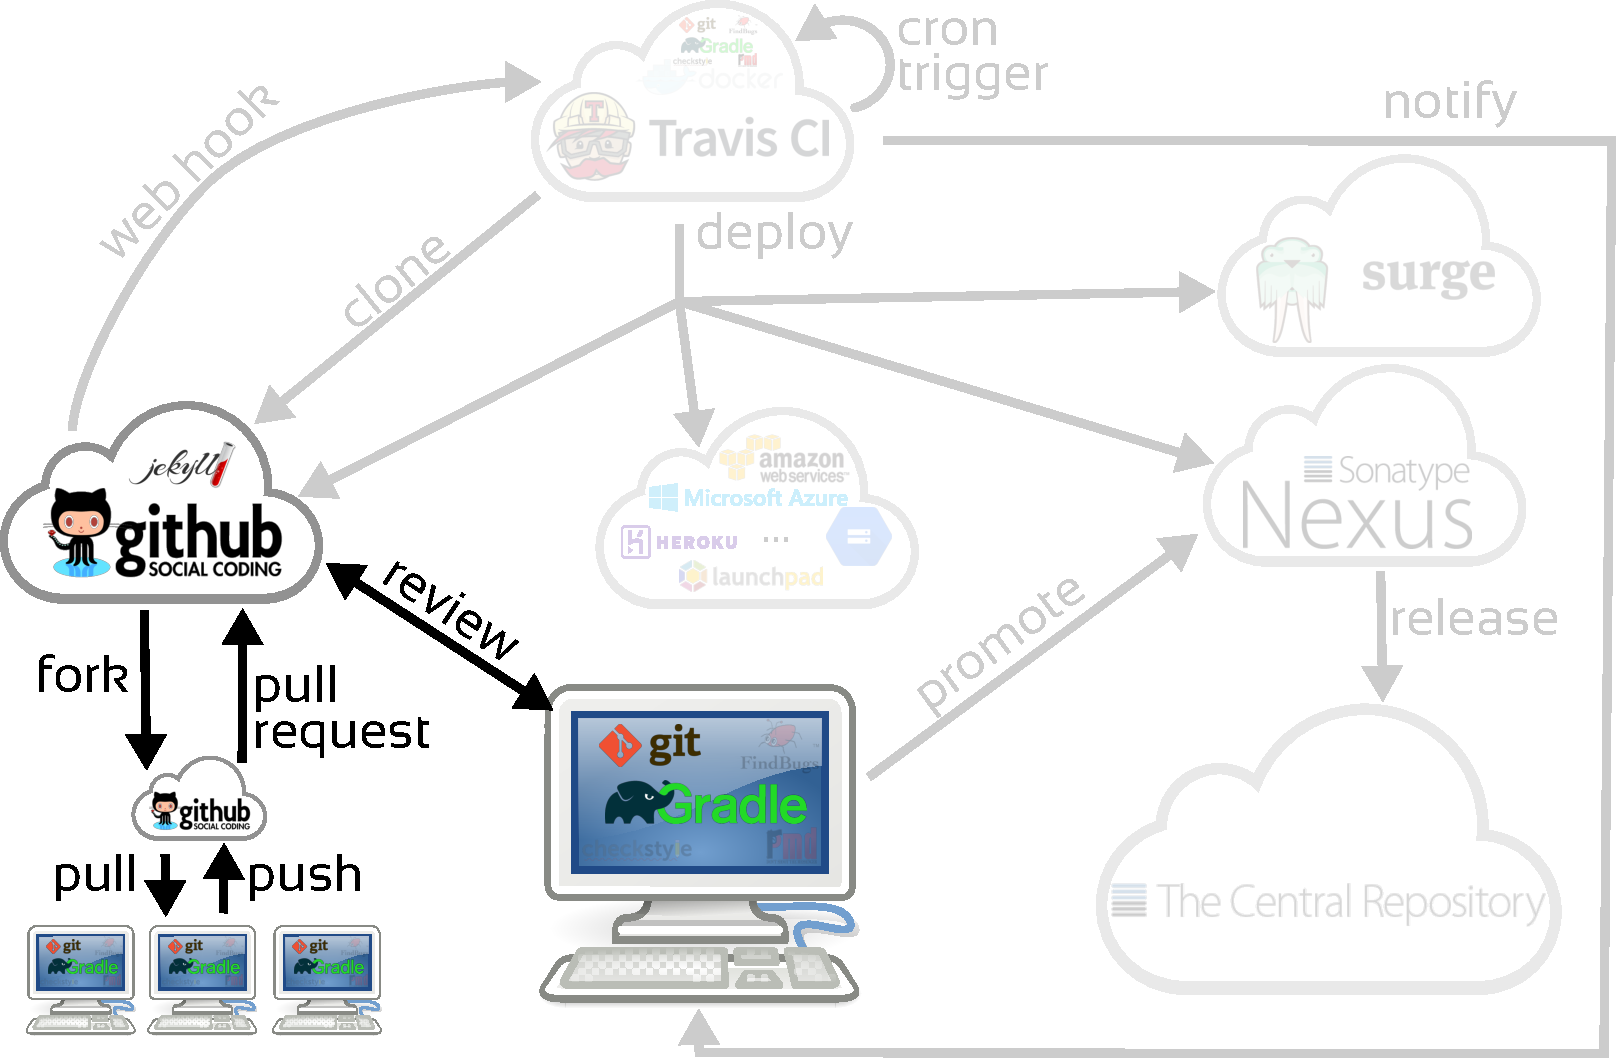
\includegraphics[width=.9\textwidth]{images/ci-gradle}
	\end{center}
\end{frame}

\begin{frame}[fragile]{The concept of dependency}
  \begin{itemize}
    \item Any software \textbf{depends} on other software
    \begin{itemize}
      \item All the runtime base libraries (think of \texttt{java.lang.* and System.*})
      \item All the other core libraries
      \item Possibly, external resources (e.g., images, sounds, translation files...)
    \end{itemize}
   \item Normally, this software depends on other software
    \begin{itemize}
      \item That depend on other software
		\begin{itemize}
			\item That depend on other software, and so on...
		\end{itemize}
    \end{itemize}
   \item A normal applications has a \textbf{tree} of dependencies
  \end{itemize}
\end{frame}

\begin{frame}[fragile]{Example: print titles}
	\begin{block}{Requirements}
		Write a program that:
		\begin{itemize}
			\item Visits TheTVDB.org (public TV Series database)
			\item Searches for a series
			\item Download the titles of all the episodes
			\item Prints them on screen
		\end{itemize}
	\end{block}
	\begin{block}{Questions}
		\begin{itemize}
			\item Estimate how much code (in Java) you'd need to write
			\item How much code can be just inherited from existing, public libraries?
		\end{itemize}
	\end{block}
\end{frame}

\begin{frame}[fragile]{Maybe less code than you may expect}
  \begin{block}{}
    \begin{minted}[fontsize=\scriptsize]{java}
package it.unibo.ci;

import ...

public final class PrintSeries {
    private static final String LANG = "it";
    private static final String SERIE = "Breaking Bad";
    private PrintSeries() {
    }
    public static void main(final String... args) throws IOException {
	final String key = IOUtils.toString(PrintSeries.class
		.getResourceAsStream("/TheTVDBAPIKey"), Charsets.UTF_8);
	final TheTVDBApi api = new TheTVDBApi(key);
	api.searchSeries("Breaking Bad", LANG).stream()
		.filter(s -> s.getSeriesName().equals(SERIE))
		.map(Series::getId)
		.flatMap(sId -> api.getAllEpisodes(sId, LANG).stream())
		.map(Episode::getEpisodeName)
		.forEach(System.out::println);
    }
}
    \end{minted}
  \end{block}
\end{frame}

\begin{frame}[fragile]{Trick revealed}
  I used a few existing libraries!
  \begin{itemize}
    \item Google Guava
    \begin{itemize}
      \item Used for referencing the UTF-8 \texttt{Charset} without using \texttt{String}s (less error-prone)
    \end{itemize}
    \item Apache Commons I/O
    \begin{itemize}
      \item Used for converting a resource stream pointing to a \texttt{String} 
    \end{itemize}
    \item Omertron's thetvdbapi
    \begin{itemize}
      \item Queries TheTVDB given a valid API key, hiding all the HTTP communication and XML parsing
    \end{itemize}
  \end{itemize}
  \begin{block}{But wait, there is more!}
    I only needed three libraries to get the job done. But are those libraries using other libraries?
  \end{block}
\end{frame}

\begin{frame}[fragile]{The actual dependency tree}
  \begin{block}{}
    \begin{minted}[fontsize=\scriptsize]{bash}
+--- com.google.guava:guava:+ -> 19.0-rc2
+--- commons-io:commons-io:+ -> 2.4
\--- com.omertron:thetvdbapi:+ -> 1.7
     +--- org.slf4j:slf4j-api:1.7.9
     \--- org.yamj:api-common:1.2
          +--- org.apache.commons:commons-lang3:3.3.2
          +--- commons-dbcp:commons-dbcp:1.4
          |    \--- commons-pool:commons-pool:1.5.4 -> 1.6
          +--- commons-pool:commons-pool:1.6
          +--- commons-codec:commons-codec:1.10
          +--- org.apache.httpcomponents:httpclient:4.3.6
          |    +--- org.apache.httpcomponents:httpcore:4.3.3
          |    +--- commons-logging:commons-logging:1.1.3
          |    \--- commons-codec:commons-codec:1.6 -> 1.10
          \--- org.slf4j:slf4j-api:1.7.9
    \end{minted}
  \end{block}
  \begin{itemize}
   \item Libraries depend on other libraries
   \item All the libraries must be in the classpath!
  \end{itemize}
\end{frame}

\begin{frame}[fragile, allowframebreaks]{Towards a dependency hell}
	This was a toy program, consisting of a single Java source file of some twenty lines of code.

	Regardless, it requires \textbf{12} external libraries in order to run.
	
	\begin{block}{Libraries explosion}
		\begin{itemize}
			\item It is very common for a non-toy project to get past 50 dependencies
			\begin{itemize}
				\item Alchemist, big but not huge, counts more than 120 dependencies
			\end{itemize}
			\item Hard to search, download and verify compatibilities by hand 
			\item Version conflicts soon arise
			\begin{itemize}
				\item one of your direct dependencies uses library \texttt{A} at version 1
				\item another uses library \texttt{A} at version 2
				\item you have a so-called transitive dependency conflict on \texttt{A}
			\end{itemize}
			\item Upgrading by hand requires, time, effort and tons of testing
		\end{itemize}
	\end{block}
	\begin{block}{Source import}
		\begin{itemize}
			\item Duplication
			\item More library code than product code
			\item Extremely difficult to update
			\item Style inconsistencies
			\item Different quality metrics
			\item Duplication
			\item Unmaintainable
		\end{itemize}
	\end{block}
	\begin{block}{Binary import (copy of jars in the repo)}
		\begin{itemize}
			\item At every update, a new jar must be included, along with all its dependencies
			\item Being a compressed binary file, its hard to write diffs
			\item Git must store a copy of the file for each version (even if very little changed actually)
			\item The repository size explodes
			\begin{itemize}
				\item Take a look at \cite{explodedrepository} for an anti-pattern
			\end{itemize}
		\end{itemize}
	\end{block}
	\begin{block}{}
		Trust me, you want an automated tool to get you out of this hell.
	\end{block}
\end{frame}

\begin{frame}[fragile]{Desiderata}
	\begin{itemize}
		\item Declarative dependency specification
		\item Automatic fetch and retrieve of the required dependencies
		\item Automatic and configurable version conflict resolution
		\item Multiple dependency scopes:
		\begin{itemize}
			\item We need JUnit for our tests, but we don't want any of our production sources to use its APIs (test scope differs from compile scope)
			\item also, we don't want to embed JUnit in our production dependency set (test scope differs from runtime scope)
			\item We need Logback \cite{logback} for our runtime, but we want our code to depend only on the SLF4J APIs for reusability (runtime scope larger than compile scope)
			\item We want ANTLR4 \cite{antlr4} for generating some source code, but we only want its runtime once this phase is concluded (custom scope)
		\end{itemize}
		\item Configurable software sources
	\end{itemize}
\end{frame}

\begin{frame}[fragile]{Possible desired code}
  \begin{block}{}
    \begin{minted}[fontsize=\scriptsize]{groovy}
repositories {
    mavenCentral()
    jCenter()
}
dependencies {
    sourceGeneration 'org.antlr:antlr4:4.7'
    compile 'org.slf4j:slf4j-api:1.7.25'
    compile 'org.antlr:antlr-runtime:3.5.2'
    testCompile 'junit:junit:4.12'
    runtime 'ch.qos.logback:logback-classic:1.2.2'
    testRuntime 'ch.qos.logback:logback-classic:1.2.2'
}
    \end{minted}
  \end{block}
\end{frame}


\begin{frame}[fragile]{Moar automation}
	Dependency management is just the \textit{first} need that arises.
	
	\begin{block}{What you really want to automatize}
		\begin{itemize}
			\item Dependency management
			\item Software compilation
			\item Test execution compilation
			\item Documentation generation
			\item Reports generation
			\item Artefacts assemblage
			\item Artefacts signing
		\end{itemize}
	\end{block}
	\begin{itemize}
		\item Everything that goes from declaring what your software needs to having it ready for deployment
		\item Except actually \textit{developing} the project
	\end{itemize}
\end{frame}

%===============================================================================
\subsection{Gradle}
%===============================================================================

\begin{frame}[fragile, allowframebreaks]{Gradle}
	\begin{block}{Idea}
		Pick the best of ``declarative'' build systems, such as Apache Maven
		\begin{itemize}
			\item Dependency resolution
			\item Rich default configuration
		\end{itemize}
		Pick the best from ``imperative'' build systems, such as Apache Ant.
		\begin{itemize}
			\item Extreme flexibility
		\end{itemize}
	\end{block}
	\begin{block}{Features}
		\begin{itemize}
			\item The build is written in a Groovy based DSL
			\item Inherits from Ant the concept of ``task''
			\item Automagic resolution of the order in which tasks should be executed
			\item Built-in dependency resolution as Maven (SBT and Ant rely on Apache Ivy)
			\item Incremental builds
			\item Parallel task execution
			\item Supports many languages (Java, Scala, Groovy are first class citizens)
			\item Maven-style extensibility via plugins
		\end{itemize}
	\end{block}
	\begin{block}{Diffusion}
		\begin{itemize}
			\item Slowly replacing Ant+Ivy and Maven as reference build system for Java and other JVM based languages
			\item Gaining momentum also in the C/C++ community (assembler, c, cpp, objective-c, and objective-cpp are set to be included in the base distribution)
			\item Selected by Google as preferred build system for Android
			\begin{itemize}
				\item Android Studio by default configures a Gradle build under the hood
			\end{itemize}
			\item Similar to SBT, arguably less tailored towards Scala
			\item Well integrated in Eclipse and (especially) IntelliJ
			\item Eclipse recently included the Gradle Buildship in the classic distribution
		\end{itemize}
	\end{block}
	\begin{block}{Details}
		\begin{itemize}
			\item Created in 2008 by Gradleware
			\item Mostly implemented in Java 5, with an outer layer in Groovy
			\item Free - both as in freedom (Apache License 2.0) and as in beer (no fees required)
			\item Source code available on GitHub
			\item Thorough documentation - though some advanced use requires some good personal initiative...
		\end{itemize}
	\end{block}
\end{frame}

\begin{frame}[fragile]{Gradle concepts}
	\begin{block}{Project - from the Gradle documentation}
			What a project represents depends on what it is that you are doing with Gradle. For example, a project might represent a library JAR or a web application. It might represent a distribution ZIP assembled from the JARs produced by other projects. \\
			A project does not necessarily represent a thing to be built.
			It might represent a thing to be done, such as deploying your application to staging or production environments.
	\end{block}
	\begin{block}{Task - from the Gradle documentation}
			Each project is made up of one or more tasks. \\
			A task represents some atomic piece of work which a build performs.\\
			This might be compiling some classes, creating a JAR, generating Javadoc, or publishing some archives to a repository.
	\end{block}
\end{frame}

\begin{frame}[fragile]{Under the hood}
	\begin{itemize}
		\item The Gradle build script is \textit{technically} a valid Groovy script (if you consider the Gradle API)
		\item Anything that has not a valid Groovy syntax is not a valid Gradle build script
		\item Groovy makes it easy to create DSLs, Gradle is built relying on such a feature
		\item Everything you write is actually proper Groovy code (method calls, closures, and so on), but (you'll see) that aspect is very nicely hidden
		\item At the high level, the feeling is to just have to configure an existing plugin, much like Maven, for most of the things you normally do
		\item When needed, it is easy to configure custom behaviour, or fiddle with the internals, in a functional or imperative fashion
	\end{itemize}
\end{frame}

\begin{frame}[fragile, allowframebreaks]{Minimal Java build}
	\begin{block}{\texttt{src/main/java/HelloWorld.java}}
		\begin{minted}[fontsize=\scriptsize]{java}
public class HelloWorld {

    public static void main(String[] args) {
        System.out.println("Hello, world!");
    }
    
}
		\end{minted}
	\end{block}
	\begin{block}{\texttt{build.gradle}}
		\begin{minted}[fontsize=\scriptsize]{groovy}
apply plugin: 'java'
		\end{minted}
	\end{block}
	Yes, it's a one-liner.
	\begin{block}{File system before the Gradle execution}
		\begin{minted}[fontsize=\scriptsize]{bash}
$ tree -A
.
|-- build.gradle
|-- src
    |-- main
        |-- java
            |-- HelloWorld.java

3 directories, 2 files
		\end{minted}
	\end{block}
	\begin{block}{Terminal}
		\begin{minted}[fontsize=\scriptsize]{bash}
$ gradle build
:compileJava
:processResources NO-SOURCE
:classes
:jar
:assemble
:compileTestJava NO-SOURCE
:processTestResources NO-SOURCE
:testClasses UP-TO-DATE
:test NO-SOURCE
:check UP-TO-DATE
:build

BUILD SUCCESSFUL

Total time: 1.024 secs
		\end{minted}
	\end{block}
	\begin{block}{File system after the execution}
		\begin{minted}[fontsize=\scriptsize]{bash}
$ tree -A
.
|-- build
|   |-- classes
|   |   |-- main
|   |       |-- HelloWorld.class
|   |-- libs
|   |   |-- 06 - Minimal Java.jar
|   |-- tmp
|       |-- compileJava
|       |-- jar
|           |-- MANIFEST.MF
|-- build.gradle
|-- src
    |-- main
        |-- java
            |-- HelloWorld.java

10 directories, 5 files
		\end{minted}
	\end{block}
	\begin{center}
		Pretty magic, huh?
	\end{center}
\end{frame}

\begin{frame}[fragile]{Let's build our toy example}
	\begin{block}{\texttt{src/main/java/it/unibo/ci/PrintBreakingBad.java}}
		\begin{minted}[fontsize=\tiny]{java}
package it.unibo.ci;

import java.io.IOException;
import org.apache.commons.io.IOUtils;
import com.google.common.base.Charsets;
import com.omertron.thetvdbapi.TheTVDBApi;
import com.omertron.thetvdbapi.model.Episode;
import com.omertron.thetvdbapi.model.Series;

public final class PrintBreakingBad {
    private static final String LANG = "it";
    private static final String SERIE = "Breaking Bad";
    private PrintBreakingBad() {
    }

    public static void main(String... args) throws ClassNotFoundException, IOException {
        final String key = IOUtils.toString(PrintBreakingBad.class.getResourceAsStream("/TheTVDBAPIKey"),
                Charsets.UTF_8);
        final TheTVDBApi api = new TheTVDBApi(key);
        api.searchSeries("Breaking Bad", LANG).stream()
            .filter(s -> s.getSeriesName().equals(SERIE))
            .map(Series::getId)
            .flatMap(s -> api.getAllEpisodes(s, LANG).stream())
            .map(Episode::getEpisodeName)
            .forEach(System.out::println);
    }
}
		\end{minted}
	\end{block}
\end{frame}

\begin{frame}[fragile]{Let's build our toy example}
	\begin{block}{\texttt{build.gradle}}
		\begin{minted}[fontsize=\scriptsize]{groovy}
apply plugin: 'java'

sourceCompatibility = "$jdkVersion"

repositories {
    mavenCentral()
}

dependencies {
    compile "com.google.guava:guava:$guavaVersion"
    compile "commons-io:commons-io:$commonsIoVersion"
    compile "com.omertron:thetvdbapi:$tvDbApiVersion"
}
		\end{minted}
	\end{block}
\end{frame}

\begin{frame}[fragile]{Let's build our toy example}
	\begin{block}{\texttt{gradle.properties}}
		\begin{minted}[fontsize=\tiny]{java}
group = it.unibo.apice
artifactId = printbbepisodes
version = 0.0.0
projectLongName = Breaking Bad Episode Titles
projectDescription = A program that fetches information about Breaking Bad on TheTVDb and prints episodes
licenseName = Apache License 2.0

jdkVersion = 1.8

commonsIoVersion = +
guavaVersion = 19.0
tvDbApiVersion = [1.6, 1.7]
		\end{minted}
	\end{block}
	\begin{block}{\texttt{settings.gradle}}
		\begin{minted}[fontsize=\tiny]{java}
rootProject.name = "$artifactId"
		\end{minted}
	\end{block}
\end{frame}

\begin{frame}[fragile]{Let's build our toy example}
	\begin{block}{\texttt{Execution}}
		\begin{minted}[fontsize=\tiny]{bash}
$ gradle clean build
:clean
:compileJava
Download https://repo1.maven.org/maven2/com/google/guava/guava/19.0/guava-19.0.pom
Download https://repo1.maven.org/maven2/com/google/guava/guava-parent/19.0/guava-parent-19.0.pom
Download https://repo1.maven.org/maven2/com/omertron/thetvdbapi/1.7/thetvdbapi-1.7.pom
Download https://repo1.maven.org/maven2/org/sonatype/oss/oss-parent/9/oss-parent-9.pom
Download https://repo1.maven.org/maven2/org/slf4j/slf4j-api/1.7.9/slf4j-api-1.7.9.pom
...many transitive dependencies after...
Download https://repo1.maven.org/maven2/commons-dbcp/commons-dbcp/1.4/commons-dbcp-1.4.jar
Download https://repo1.maven.org/maven2/commons-pool/commons-pool/1.6/commons-pool-1.6.jar
Download https://repo1.maven.org/maven2/commons-codec/commons-codec/1.10/commons-codec-1.10.jar
Download https://repo1.maven.org/maven2/org/apache/httpcomponents/httpclient/4.3.6/httpclient-4.3.6.jar
Download https://repo1.maven.org/maven2/org/apache/httpcomponents/httpcore/4.3.3/httpcore-4.3.3.jar
:processResources
:classes
:jar
:assemble
:compileTestJava UP-TO-DATE
:processTestResources UP-TO-DATE
:testClasses UP-TO-DATE
:test UP-TO-DATE
:check UP-TO-DATE
:build

BUILD SUCCESSFUL

Total time: 9.002 secs
		\end{minted}
	\end{block}
\end{frame}

\begin{frame}[fragile]{Dependency management in Gradle}
	\begin{itemize}
		\item Dependencies in Gradle can be specified by defining
		\begin{itemize}
			\item Where to retrieve software (Maven Central and JCenter are first class citizens)
			\item The list of dependencies for each scope
			\item Some scopes import other scopes (e.g. \texttt{runtime} by default contains the whole \texttt{compile} scope)
		\end{itemize}
		\item Dependencies can be specified with a specific version, a version range, or using \texttt{+} as ``latest''
		\begin{itemize}
			\item With \texttt{1.+} meaning ``the latest version starting with \texttt{1.}''
			\item Prefer specific versions or ranges (you \textbf{must} test them)
		\end{itemize}
		\item Transitive dependencies are resolved automatically (if available in the repository, of course)
		\item Specifying the \texttt{sourceCompatibility} is not required, but recommended
	\end{itemize}
\end{frame}

\begin{frame}[fragile]{Tests as part of the build}
	As you can see from the output of the previous case, the tests are executed by default for every build!
	\begin{block}{Tests and Gradle, how to:}
		\begin{itemize}
			\item Add the libraries you need to the appropriate dependency scope
			\item Put your test sources in \texttt{src/test/nameofyourlanguage}
		\end{itemize}
	\end{block}
	\begin{block}{\texttt{build.gradle} that enables and uses JUnit}
		\begin{minted}[fontsize=\scriptsize]{groovy}
apply plugin: 'java'
repositories {
    mavenCentral()
}
dependencies {
    testCompile 'junit:junit:4.12'
}
		\end{minted}
	\end{block}
\end{frame}
\begin{frame}[fragile, allowframebreaks]{Multi-language build}
	\begin{block}{File system before the execution}
		\begin{minted}[fontsize=\scriptsize]{bash}
$ tree -A
.
|-- build.gradle
|-- src
    |-- main
        |-- groovy
        |   |-- HelloGroovy.groovy
        |-- java
        |   |-- HelloWorld.java
        |   |-- TestXtend.xtend
        |-- scala
            |-- HelloScala.scala

5 directories, 5 files
		\end{minted}
	\end{block}
	\begin{block}{\texttt{src/main/groovy/HelloGroovy.groovy}}
		\begin{minted}[fontsize=\scriptsize]{groovy}
println "Hello, Groovy"
		\end{minted}
	\end{block}
	\begin{block}{\texttt{src/main/java/HelloWorld.java}}
		\begin{minted}[fontsize=\scriptsize]{java}
public class HelloWorld {

    public static void main(String... args) {
        System.out.println("Hello, world!");
    }
    
}
		\end{minted}
	\end{block}
	\begin{block}{\texttt{src/main/java/TestXtend.xtend}}
		\begin{minted}[fontsize=\scriptsize]{xtend}
class TestXtend {
  def static void main(String... args) {
    println("Hello Xtend")
  }
}
		\end{minted}
	\end{block}
	\begin{block}{\texttt{src/main/scala/HelloScala.scala}}
		\begin{minted}[fontsize=\scriptsize]{scala}
object HelloScala extends App  {
    println("Hello Scala")
}
		\end{minted}
	\end{block}
	\begin{block}{\texttt{build.gradle}}
		\begin{minted}[fontsize=\scriptsize]{groovy}
plugins {
  id "org.xtext.xtend" version "1.0.0"
}
apply plugin: 'java'
apply plugin: 'scala'
apply plugin: 'groovy'

repositories {
    mavenCentral()
}

dependencies {
    compile 'org.scala-lang:scala-library:2.12.2'
    compile 'org.codehaus.groovy:groovy:2.3.7'
    compile 'org.eclipse.xtend:org.eclipse.xtend.lib:2.9.0'
}
		\end{minted}
	\end{block}
	\begin{block}{\texttt{Execution}}
		\begin{minted}[fontsize=\tiny]{bash}
$ gradle clean build
:clean
:generateXtext
:compileJava
:compileGroovy
:compileScala
:processResources NO-SOURCE
:classes
:jar
:assemble
:generateTestXtext NO-SOURCE
:compileTestJava NO-SOURCE
:compileTestGroovy NO-SOURCE
:compileTestScala NO-SOURCE
:processTestResources NO-SOURCE
:testClasses UP-TO-DATE
:test NO-SOURCE
:check UP-TO-DATE
:build

BUILD SUCCESSFUL

Total time: 10.627 secs
		\end{minted}
	\end{block}
	\begin{block}{Build folder after the execution}
		\begin{minted}[fontsize=\tiny]{bash}
$ tree -A build
build
|-- classes
|   |-- main
|       |-- HelloGroovy.class
|       |-- HelloScala.class
|       |-- HelloScala$.class
|       |-- HelloScala$delayedInit$body.class
|       |-- HelloWorld.class
|       |-- TestXtend.class
|-- java
|   |-- main
|-- libs
|   |-- 02-multilang.jar
|-- tmp
|   |-- compileGroovy
|   |   |-- groovy-java-stubs
|   |-- compileJava
|   |-- compileScala
|   |-- jar
|   |   |-- MANIFEST.MF
|   |-- scala
|       |-- compilerAnalysis
|           |-- compileScala.analysis
|           |-- compileScala.analysis.relations
|-- xtend
    |-- main
        |-- TestXtend.java
15 directories, 11 files
		\end{minted}
	\end{block}
\end{frame}


\begin{frame}[fragile]{Build system as dependency}
	If you rely on a build system to build your project, then \textbf{the build system itself is a dependency}!
	\begin{itemize}
		\item Different versions may produce a different outcome
		\item Old versions may not work
		\item Newer version may stop working
		\item The build system is as any other dependency!
	\end{itemize}
	\begin{block}{The Gradle wrapper}
		Gradle provides a builtin wrapper task:
		\begin{itemize}
			\item Downloads a gradle core jar and a few settings files
			\item Those file must be added to the tracker
			\item \texttt{gradle wrapper --gradle-version 3.1} downloads version 3.1
			\item \texttt{./gradlew <task>} runs \texttt{<task>} with that exact version
		\end{itemize}
	\end{block}
\end{frame}

\begin{frame}[fragile]{IDE integration}
	IntelliJ integration is straightforward, no additional configuration is required.
	
	A Gradle integration plugin is included in the Eclipse distribution (Buildship).
	\begin{block}{\texttt{build.gradle}}
		\begin{minted}[fontsize=\scriptsize]{groovy}
apply plugin: 'eclipse'

eclipse {
    classpath {
        downloadJavadoc = true
        downloadSources = true
    }
}
		\end{minted}
	\end{block}
	Downloads from the repositories also sources and javadocs and feeds them to Eclipse: much easier to develop...
\end{frame}

\begin{frame}[fragile]{How the world looks like now}
	\begin{center}
		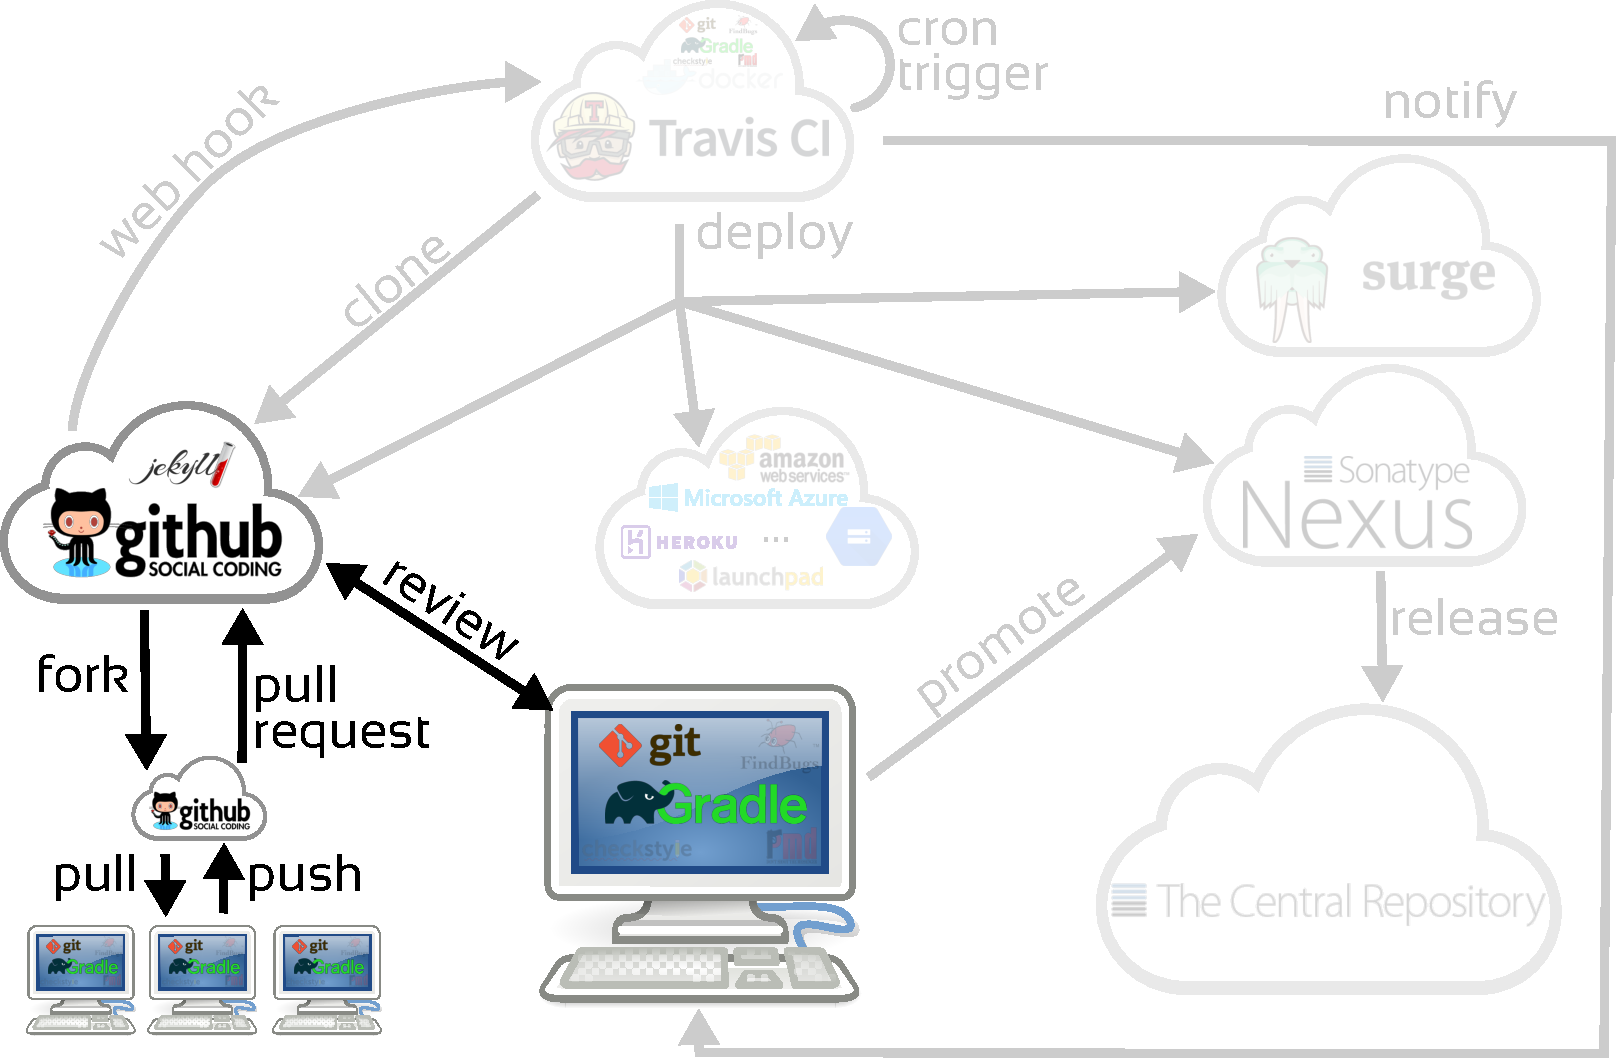
\includegraphics[width=.9\textwidth]{images/ci-gradle}
	\end{center}
\end{frame}

%===============================================================================
\subsection{Code quality control}
%===============================================================================

\begin{frame}[fragile]{How will the world look like shortly}
	\begin{center}
		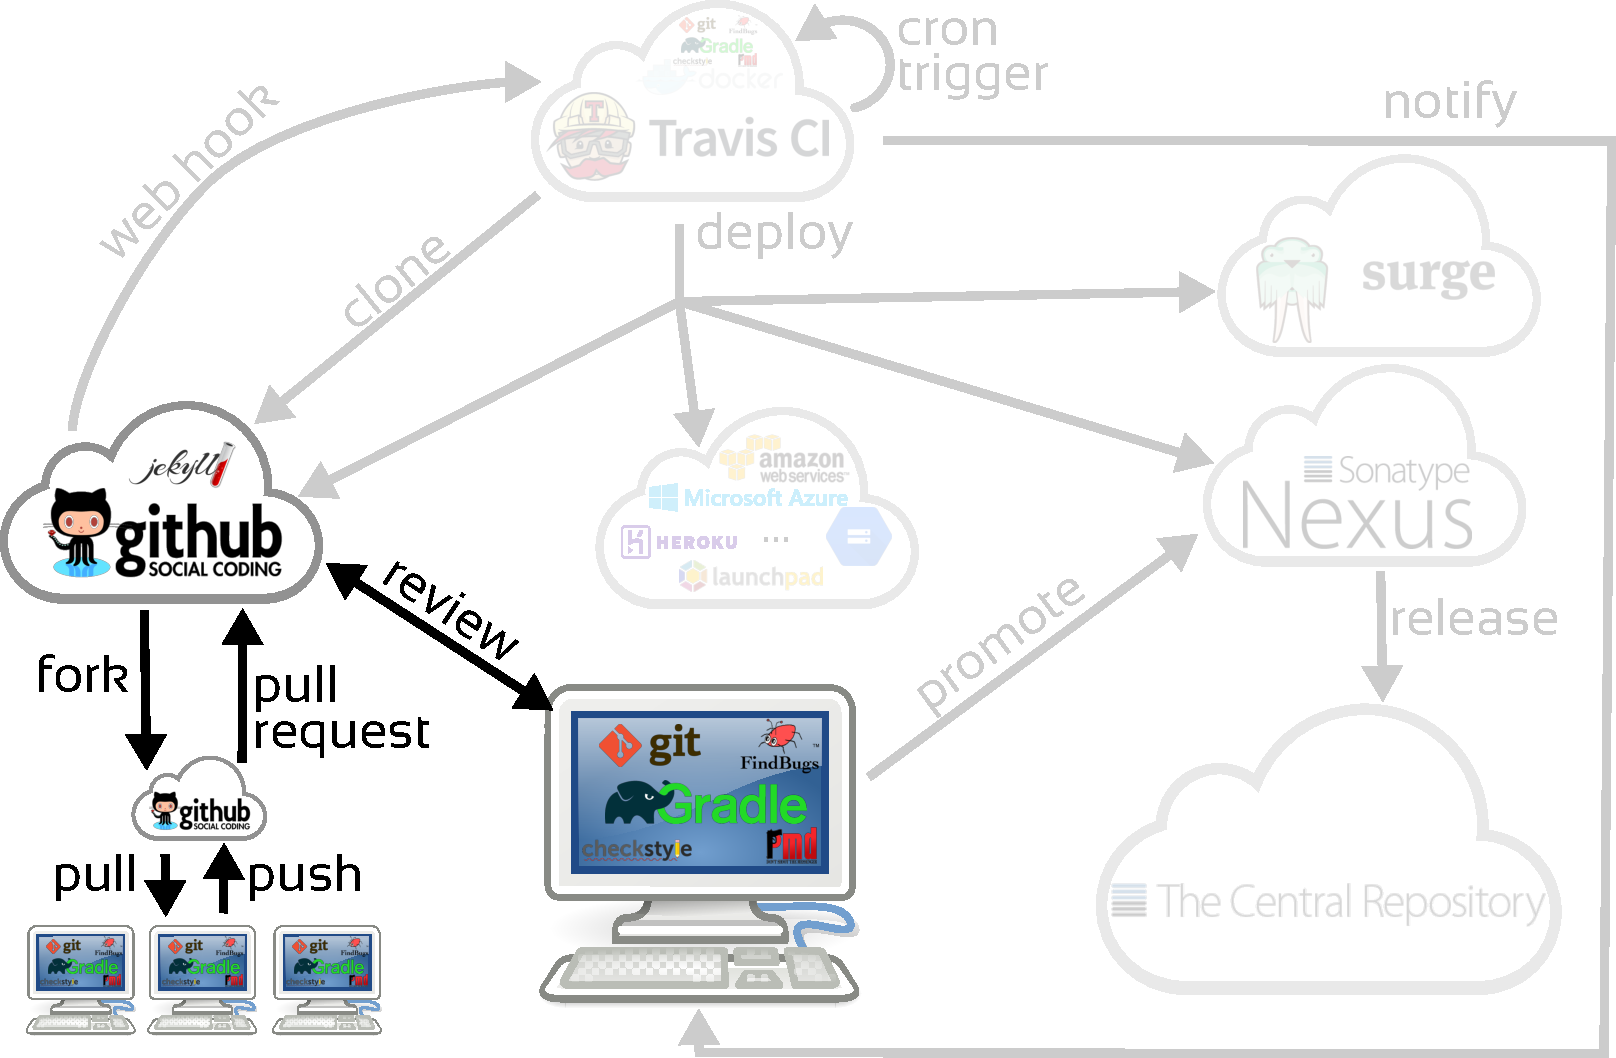
\includegraphics[width=.9\textwidth]{images/ci-codequality}
	\end{center}
\end{frame}

\begin{frame}[fragile]{Automatic code quality control}
	\begin{block}{Why}
		\begin{itemize}
			\item Immediately spot subtle bugs
			\item Early spot sub-optimal code (singular fields, missing finals...)
			\item Enforce encapsulation, spot cut/pastes (normally sign of bad design choices)
			\item Use a coherent style across your code
			\item Prevent style-change commits (``The Leopard commits'')
			\item Particularly important if there are many developers!
		\end{itemize}
	\end{block}
\end{frame}

\begin{frame}[fragile]{Automatic code quality control}
	\begin{block}{How}
		\begin{itemize}
			\item FindBugs
			\begin{itemize}
				\item Analyzes the bytecode searching for bugs
			\end{itemize}
			\item PMD
			\begin{itemize}
				\item Source code analyzer for common programming flaws
				\item Finds suspect cut/paste (CPD module)
				\item Works for Java, Javascript, PLSQL, Velocity, XML, XSL
			\end{itemize}
			\item Checkstyle
			\begin{itemize}
				\item Forces code standard (indentation, formatting, Javadoc...)
				\item Can be configured for working with arbitrary files
			\end{itemize}
			\item Codacy
			\begin{itemize}
				\item Web based
				\item scala-meta is available for Scala
			\end{itemize}
		\end{itemize}
	Plugins available for Gradle, Eclipse and IntelliJ
	\end{block}
\end{frame}

\begin{frame}[fragile]{Code quality control advices}
	\begin{itemize}
		\item Ship the code checkers configuration files with your distribution
		\begin{itemize}
			\item Usually just one or two XML files
		\end{itemize}
		\item Make your IDE plugins configuration \textit{match exactly} your build automation tool configuration
		\item Always track the IDE configuration with your SCM
		\begin{itemize}
			\item New developers will import the configuration automatically if they have plugins installed
			\item If a bad developer tries to change the configuration, you can spot it from the commit change set
		\end{itemize}
		\item Pick the rule configuration that suits your project
		\begin{itemize}
			\item Some rules are controversial at least
			\item Some rule have default arbitrary limits
			\item Alchemist rules come from several years of tuning, fill free to use them
		\end{itemize}
		\item Require your developers to adhere
	\end{itemize}
\end{frame}

\begin{frame}[fragile]{How does the world look like now}
	\begin{center}
		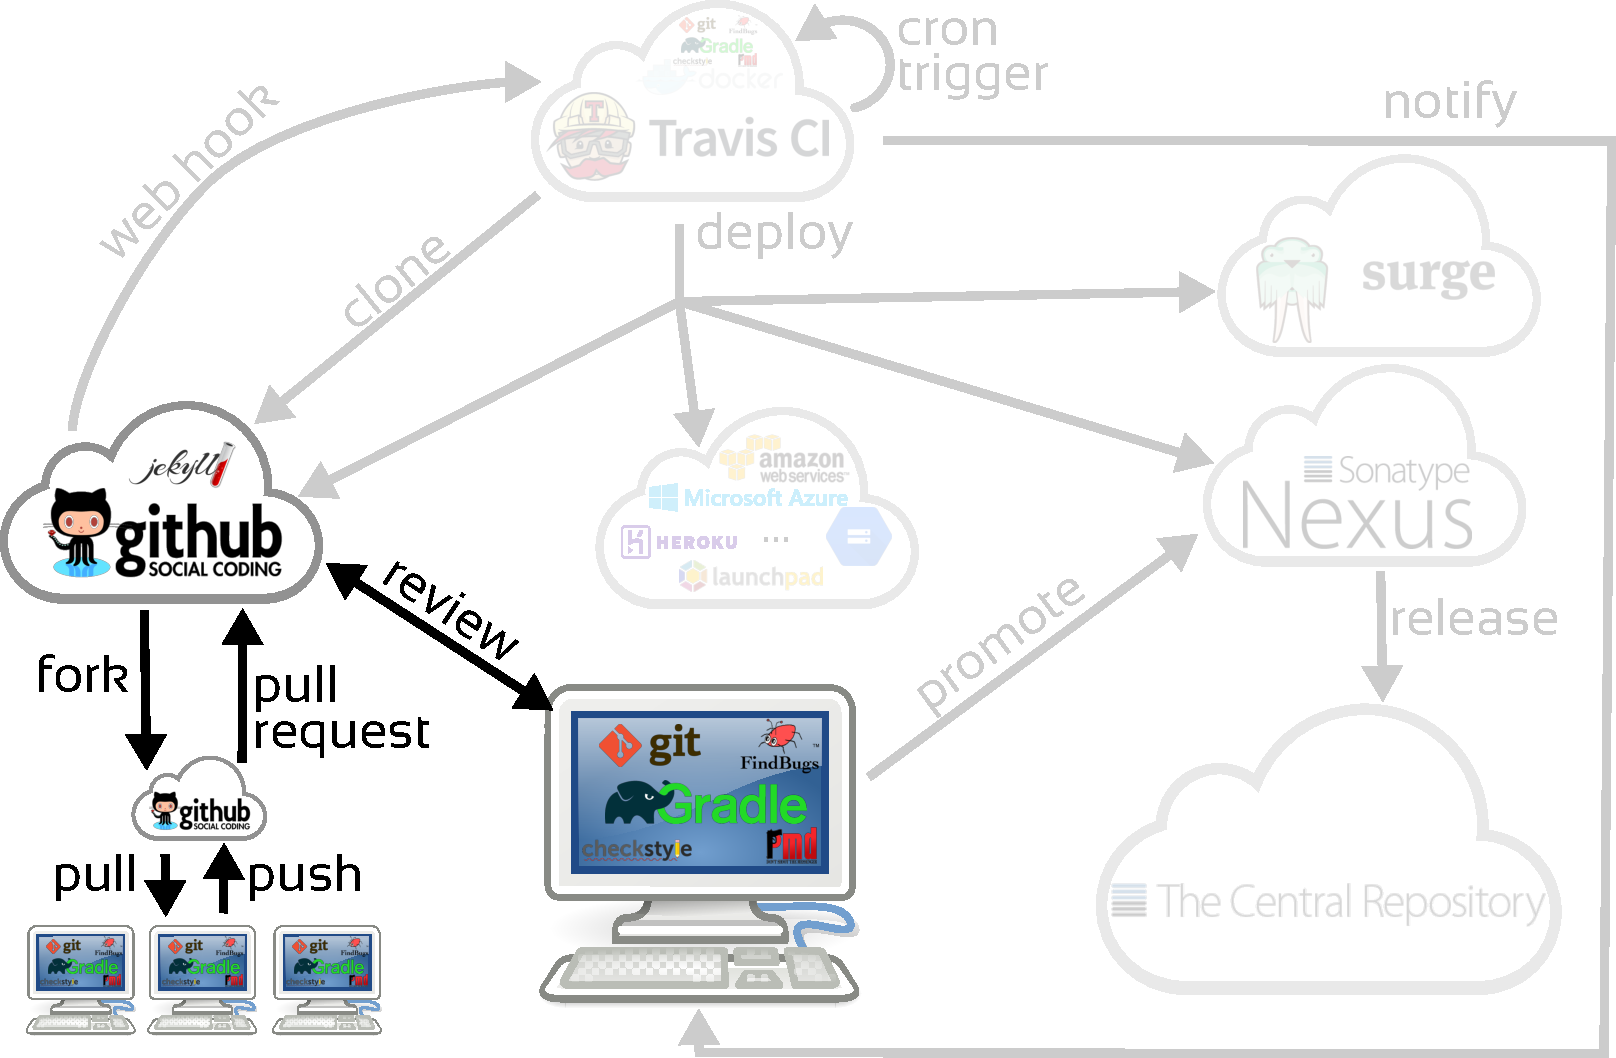
\includegraphics[width=.9\textwidth]{images/ci-codequality}
	\end{center}
\end{frame}

%===============================================================================
%===============================================================================
\section{Continuous integration}
%===============================================================================
%===============================================================================

%===============================================================================
\subsection{Travis CI}
%===============================================================================

\begin{frame}[fragile]{How will the world look like shortly}
	\begin{center}
		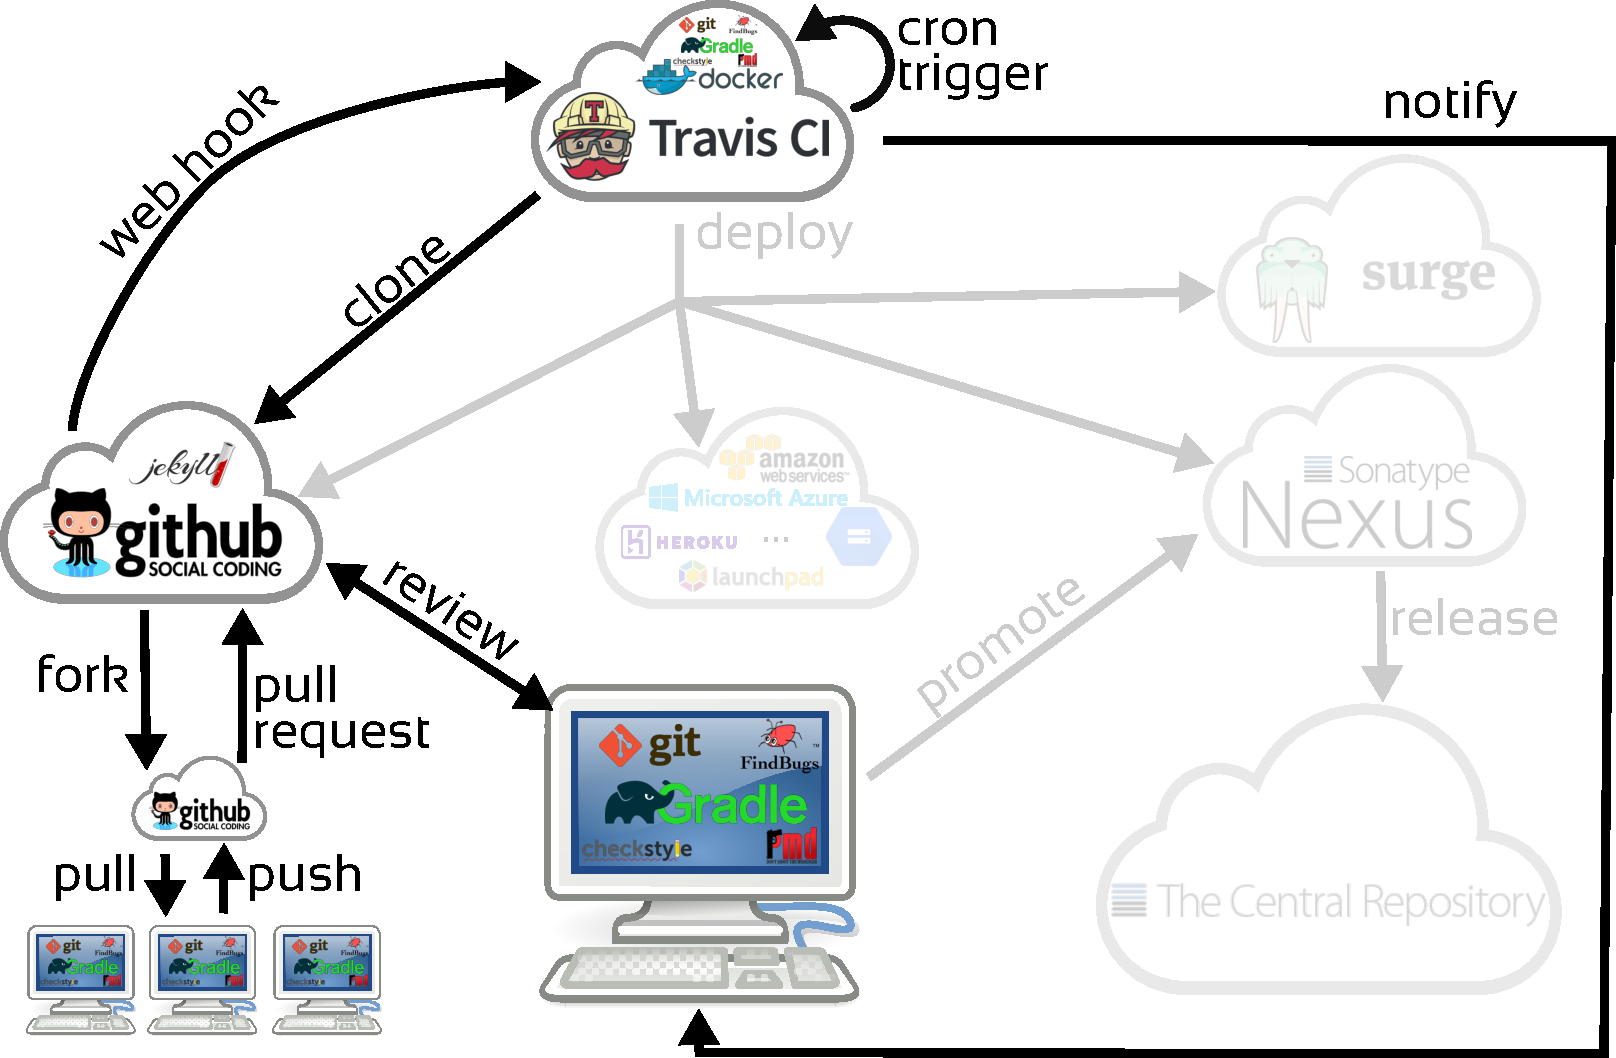
\includegraphics[width=.9\textwidth]{images/ci-travis}
	\end{center}
\end{frame}

\begin{frame}[fragile, allowframebreaks]{Summary}
	\begin{block} {We got}
		\begin{itemize}
			\item Teamwork tools
			\item Proficient teamwork strategies
			\item Project repositories
			\item Dependency management
			\item Tests integrated in the build
			\item Code quality control
			\item Automatic production of the artifacts
			\item Automatic production of reports
		\end{itemize}
	\end{block}
	\begin{block} {We miss}
		\begin{itemize}
			\item Execute the whole build for every change
			\begin{itemize}
				\item Doing it locally makes development too slow, defeating the purpose of saving development time
			\end{itemize}
			\item Execute the tests in a fresh environment, resembling the production environment
			\begin{itemize}
				\item We would need to clone a fresh VM, run the build there, then throw it away
			\end{itemize}
			\item Automatic deployment
		\end{itemize}
	\end{block}
\end{frame}

\begin{frame}[fragile]{Continuous Integration software}
	Software that promotes the practice of continuous integration
	\begin{itemize}
		\item Runs a build for every change in the project
		\item Prepares fresh environments where the builds are hosted
		\item Notifies the results, e.g. if a failure occurs
		\item Provides tools for deploying the produced artifacts
	\end{itemize}
	Hosted CI with free plans for open source projects are blossoming:
	\scriptsize
	\begin{itemize}
		\item Circle CI
		\item Codefresh
		\item Codeship
		\item drone.io
		\item Pipelines
		\item Travis CI
		\item Wercker
		\item ...
	\end{itemize}
\end{frame}

\begin{frame}[fragile]{Travis CI}
	\begin{itemize}
		\item Web based
		\item Well integrated with GitHub
		\begin{itemize}
			\item Build results are displayed in the repo without intervention
			\item Automatic build of any pull request
		\end{itemize}
		\item Free for open source projects
		\item Cronjobs
		\item Build instances based on Docker
		\item Project-local configuration via YAML (in the \texttt{.travis.yml} file)
		\item Out of the box support for Gradle
		\item Dozens of deployment targets
	\end{itemize}
\end{frame}

\begin{frame}[fragile]{How it works}
	\begin{itemize}
		\item A web-hook can be registered to your GitHub repository that triggers Travis CI at each new commit
		\item Travis CI starts a pristine appropriate environment
		\begin{itemize}
			\item Can be a container or a full virtual machine, depending on whether \texttt{sudo} is required \cite{travisbuild}
		\end{itemize}
		\item The project gets cloned
		\item The system is configured as per \texttt{.travis.yml} settings
		\item The configured commands are executed
		\item The configured deployments are performed
		\item If necessary, project managers are informed of the build status
	\end{itemize}
\end{frame}

\begin{frame}[fragile]{Minimal Travis configuration}
	\begin{block}{\texttt{.travis.yml}}
		\begin{minted}[fontsize=\scriptsize]{yaml}
language: java
		\end{minted}
	\end{block}
	\begin{enumerate}
		\item Automatically searches for \texttt{build.gradle}
		\item If found and \texttt{gradlew} is present runs
		\begin{enumerate}
			\item \texttt{./gradlew assemble}
			\item \texttt{./gradlew check}
		\end{enumerate}
		\item Otherwise runs the same commands with the version of Gradle pre-installed on the instance
	\end{enumerate}
	The command to be executed can be configured manually (recommended)
	\begin{block}{\texttt{.travis.yml}}
		\begin{minted}[fontsize=\scriptsize]{yaml}
language: java
script:
  - './gradlew clean build'
		\end{minted}
	\end{block}
	Further documentation on building Java-based projects is available \cite{travisjava}
\end{frame}

\begin{frame}[fragile]{How will the world looks like noe}
	\begin{center}
		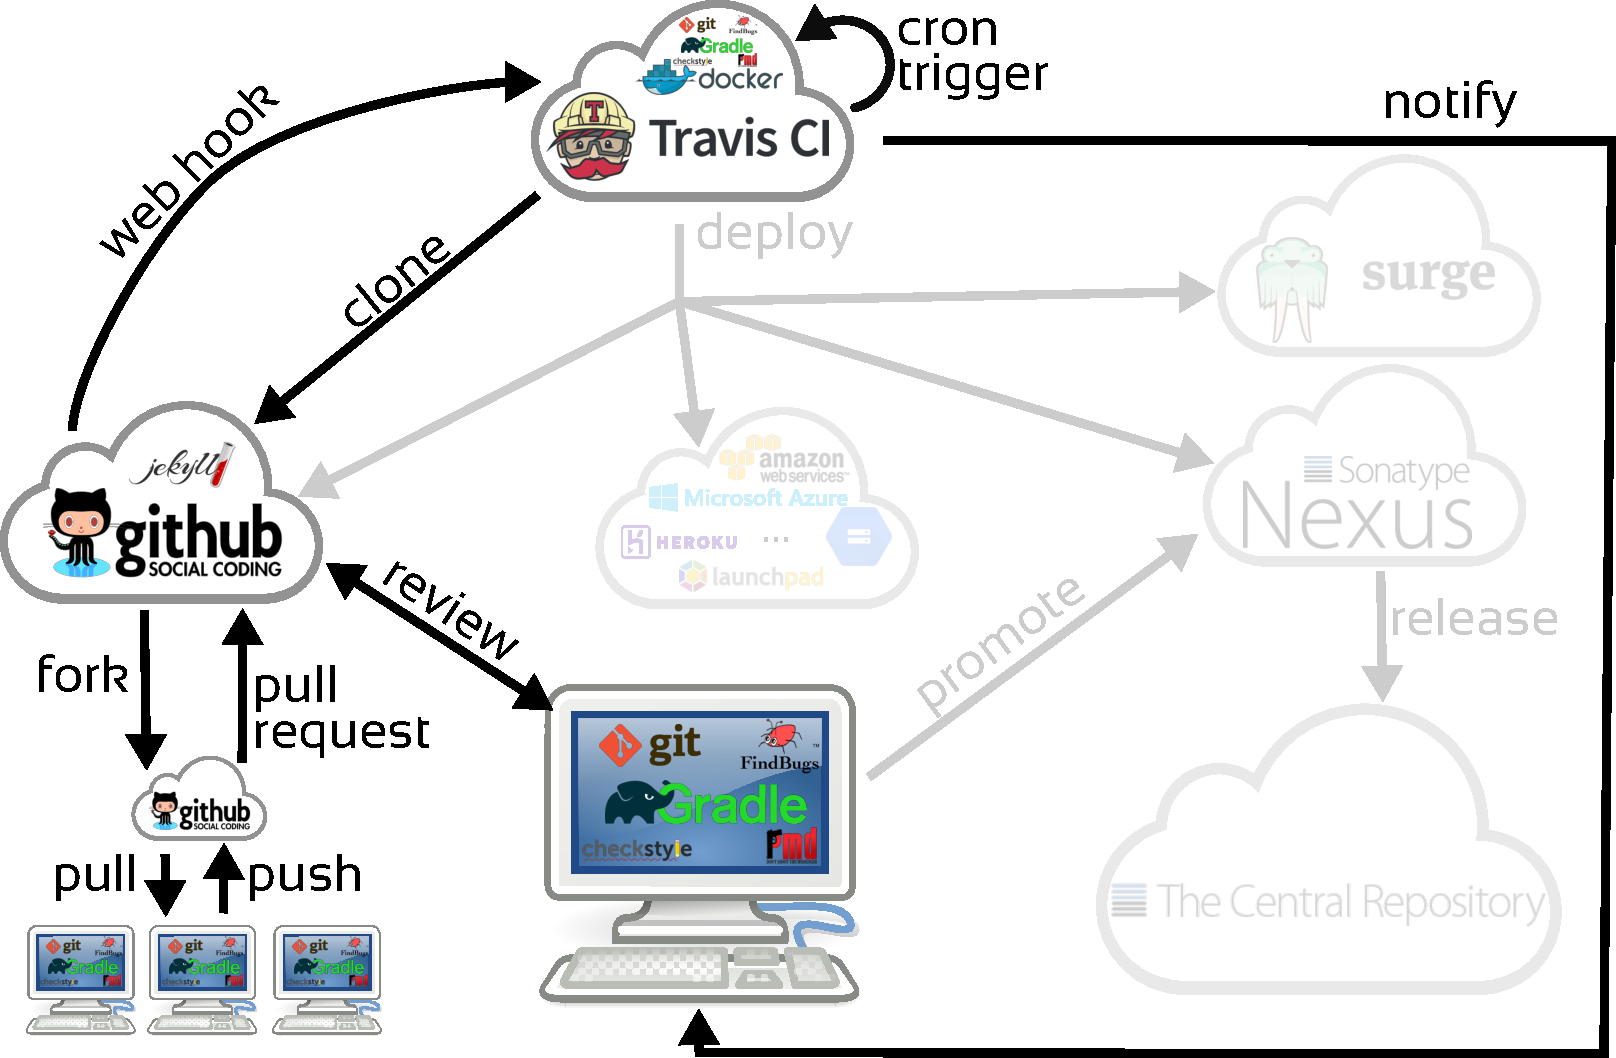
\includegraphics[width=.9\textwidth]{images/ci-travis}
	\end{center}
\end{frame}

%===============================================================================
\subsection{Deployment}
%===============================================================================

\begin{frame}[fragile]{How will the world look like shortly}
	\begin{center}
		\includegraphics[width=.9\textwidth]{images/ci}
	\end{center}
\end{frame}

\begin{frame}{Travis deployments}
	Travis CI supports deployment on a variety of targets. Two examples:
	\begin{enumerate}
		\item GitHub releases
		\begin{itemize}
			\item Creates a new download section on GitHub
			\item Great for storing executable versions (e.g. ``fat jars'')
			\item Nice automatic deployment examples are available in the Alchemist \cite{alchemist-travis} and Protelis \cite{protelis-travis} build configurations
		\end{itemize}
		\item surge.sh hosting
		\begin{itemize}
			\item Uploads a static web page on a surge.sh page
			\item Very handy for web based documentation (e.g. Javadoc)
			\item Nice automatic deployment examples are available in the Alchemist \cite{alchemist-travis} and Protelis \cite{protelis-travis} build configurations
		\end{itemize}
	\end{enumerate}
	Details on how to configure the deployments are provided in the Travis documentation \cite{travisdeploy}.
\end{frame}


\begin{frame}[fragile]{Online repositories}
	The deployment of your software greatly varies depending on who's destined to.
	
	\begin{block}{Making the software easy to use}
		\begin{itemize}
			\item Very common by-product (and sometimes product) of academic research
			\item Just shipping source code on GitHub and / or publishing jar files on a random server \textbf{is not enough}
			\item Especially for libraries or middleware, it is \textbf{way} better to provide a proper repository, where other projects can just point to and import the product as Gradle / Maven / Ant / Ivy \textit{dependency}
			\item Public services exist that offer a free and reliable repository
		\end{itemize}
	\end{block}
\end{frame}

\begin{frame}[fragile]{OSSRH --- aka Maven Central}
	\begin{itemize}
		\item Offered and managed by Sonatype
		\item Default software source for Maven builds
		\item Trivial to setup with any other build automation tool
		\item De-facto standard
		\item No-retract policy: if you publish an artifact, you cannot modify it, no exception allowed
		\item Gets copied from other repositories, e.g. jCenter
		\item Artifact staging and release through an instance of Sonatype Nexus
		\item Artifacts have a product name and belong to a group
		\item A Sonatype JIRA account and digital signature is required to manage a group
		\item Digital signature on artifacts required
		\item Strict quality control: sources and documentation must be provided
		\item See: \url{http://central.sonatype.org/pages/ossrh-guide.html}
	\end{itemize}
\end{frame}

\begin{frame}[fragile]{No retract? What if I make a mistake?}
	\begin{block}{Short answer}
		Your error will remain in the repositories forever and you will never able to fix it, you will need to create a new official release with a different version number.
	\end{block}
	\begin{block}{Anecdotal evidence of why this is good}
		In March 2016, Azer Koçlu unpublished more than 250 of his modules from NPM, which is a popular package manager used by Javascript projects to install dependencies, because he was asked to rename the module ``Kik'', whose name is the same of an instant messaging app that wanted to publish a homonym module.
		
		Unfortunately, one of those dependencies was \texttt{left-pad}, an 11 lines long Javascript module, used by thousands of projects. This brought breackages throughout many Javascript products (most notably Node and Babel). NPM had to un-unpublish \texttt{left-pad}.
		
	\end{block}
\end{frame}

\begin{frame}[fragile]{Deployment automatization}
	We have our artifacts, automatically tested and compiled (at least) every day on our nice automatic build / test / integration framework.
	
	We also want to have automatic deployment to OSSRH, so we need:
	\begin{enumerate}
		\item Generation of all required artifacts: a sources jar file and a javadoc jar file
		\item An OSSRH account
		\item A GPG signature of all these artifacts
		\item Creation of a \texttt{pom.xml} file
		\item Automatic publication in our target repository
		\item Release of final versions of our software
		\begin{itemize}
			\item Can be automated, but I prefer to have a manual check if there is a no-retract policy
		\end{itemize}
	\end{enumerate}
\end{frame}

\begin{frame}[fragile]{Automatize artifact creation}
	Very easy in Gradle:
	\begin{itemize}
		\item A task that runs after classes are compiled (to be sure we don't pack non-compiling stuff) that fits in a jar all the source code
		\item A task that runs after the Javadoc has been generated, and compresses it in a jar file
		\item Configure Gradle to add those files to the generated artifacts
	\end{itemize}
	\begin{block}{In \texttt{build.gradle}}
		\begin{minted}[fontsize=\scriptsize]{groovy}
task sourcesJar(type: Jar, dependsOn:classes) {
     classifier = 'sources' 
     from sourceSets.main.allSource 
} 
task javadocJar(type: Jar, dependsOn:javadoc) { 
     classifier = 'javadoc' 
     from javadoc.destinationDir 
} 
artifacts { 
     archives sourcesJar 
     archives javadocJar 
}
		\end{minted}
	\end{block}
\end{frame}

\begin{frame}[fragile]{OSSRH account}
	\begin{enumerate}
		\item Create and publish your own GPG key
		\begin{itemize}
			\item This is \textbf{personal}, and must not be shared
			\item Good setup guide available at: \\ \scriptsize{\url{http://central.sonatype.org/pages/working-with-pgp-signatures.html}}
		\end{itemize}
		\item Create a new account on Sonatype's Jira
		\item Create a new ticket, requesting a new group or to be added to an existing one
		\item In about two working days, you will get access to the repository, and your (signed) artifacts will be considered valid
	\end{enumerate}
\end{frame}

\begin{frame}[fragile]{Automatically sign the artifacts}
	This is the trickies part.
	\begin{itemize}
		\item Signing requires your \textbf{private} key to be exported to the build instance
		\begin{itemize}
			\item If the Travis build instance can download it, everybody can
		\end{itemize}
		\item It must be encrypted, and the instance must know how to decrypt it
		\begin{itemize}
			\item But nobody else may be able to
		\end{itemize}
		\item In short: use the instance public key to encrypt it 
		\item (a secure build it's actually more complicated than just this)
	\end{itemize}
	Once the system is configured with the private GPG key, Gradle can be told to automatically sign and upload artifacts to Maven Central
\end{frame}

\begin{frame}[fragile]{Summary of the whole process}
	\begin{center}
		\includegraphics[width=.9\textwidth]{images/ci}
	\end{center}
\end{frame}

\section*{Bonus track}

\begin{frame}[fragile]{Picking version numbers}
	\begin{quote}
		Without compliance to some sort of formal specification, version numbers are essentially useless for dependency management. By giving a name and clear definition to the above ideas, it becomes easy to communicate your intentions to the users of your software.
		\begin{flushright}
			\normalfont{--- Semantic Versioning 2.0.0 (\url{http://semver.org/})}
		\end{flushright}
	\end{quote}
	\begin{block}{Semantic versioning}
		\begin{itemize}
			\item Formally described, with RFC-style wording
			\item Three levels plus optional: \texttt{MAJOR.MINOR.PATCH[-OTHER]}
			\begin{itemize}
				\item \texttt{MAJOR} --- Any incompatible API change
				\item Major \texttt{0} is for initial development: anything may change at any time.
				\item \texttt{MINOR} --- Add functionality in a backwards-compatible manner
				\item \texttt{PATCH} --- Backwards-compatible bug fixes
				\item \texttt{OTHER} --- Optionally decorates the version with additional information.
			\end{itemize}
		\end{itemize}
	\end{block}
\end{frame}





\section*{\refname}
%===============================================================================
\begin{frame}[allowframebreaks]
  \frametitle{\refname}
  \scriptsize
  \bibliographystyle{alpha}
  \bibliography{bibliography}
\end{frame}
\section*{\refname}




\end{document}